\documentclass[a4paper]{article}
\usepackage{booktabs}
%% Language and font encodings
\usepackage[spanish]{babel}
\usepackage[utf8]{inputenc}
% Ajustes de traducciones y nombres en español
\addto\captionsspanish{%
      \renewcommand{\contentsname}{Contenido}%
      \renewcommand{\listfigurename}{Lista de figuras}%
      \renewcommand{\listtablename}{Lista de tablas}%
      \renewcommand{\tablename}{Tabla}%
      \renewcommand{\figurename}{Figura}%
      \renewcommand{\abstractname}{Resumen}%
      \renewcommand{\refname}{Referencias}%
}
\selectlanguage{spanish}
\usepackage[T1]{fontenc}

%% Sets page size and margins
\usepackage[a4paper,top=3cm,bottom=2cm,left=3cm,right=3cm,marginparwidth=1.75cm]{geometry}

%% Useful packages
\usepackage{amsmath}
\usepackage{graphicx}
\usepackage{caption}
\usepackage{url}
\usepackage{multirow}
\usepackage{float}        % opcion [H] para forzar posicion exacta de floats
\usepackage{placeins}     % \FloatBarrier: evita que floats crucen la barrera
\usepackage{tikz}
\usetikzlibrary{arrows.meta, positioning, shapes.geometric}
\usepackage{listings}
\usepackage{xcolor}

% Configuracion de listings para codigo
\lstset{
    basicstyle=\ttfamily\small,
    breaklines=true,
    frame=single,
    numbers=left,
    numberstyle=\tiny\color{gray},
    keywordstyle=\color{blue},
    commentstyle=\color{green!50!black},
    stringstyle=\color{red!60!black},
    showstringspaces=false,
    tabsize=4,
    language=Python,
    literate=
        {á}{{\'a}}1 {é}{{\'e}}1 {í}{{\'i}}1 {ó}{{\'o}}1 {ú}{{\'u}}1
        {Á}{{\'A}}1 {É}{{\'E}}1 {Í}{{\'I}}1 {Ó}{{\'O}}1 {Ú}{{\'U}}1
        {à}{{\`a}}1 {è}{{\`e}}1 {ì}{{\`i}}1 {ò}{{\`o}}1 {ù}{{\`u}}1
        {À}{{\`A}}1 {È}{{\`E}}1 {Ì}{{\`I}}1 {Ò}{{\`O}}1 {Ù}{{\`U}}1
        {ä}{{\"a}}1 {ë}{{\"e}}1 {ï}{{\"i}}1 {ö}{{\"o}}1 {ü}{{\"u}}1
        {Ä}{{\"A}}1 {Ë}{{\"E}}1 {Ï}{{\"I}}1 {Ö}{{\"O}}1 {Ü}{{\"U}}1
        {â}{{\^a}}1 {ê}{{\^e}}1 {î}{{\^i}}1 {ô}{{\^o}}1 {û}{{\^u}}1
        {Â}{{\^A}}1 {Ê}{{\^E}}1 {Î}{{\^I}}1 {Ô}{{\^O}}1 {Û}{{\^U}}1
        {ã}{{\~a}}1 {ñ}{{\~n}}1
        {Ã}{{\~A}}1 {Ñ}{{\~N}}1
        {œ}{{\oe}}1 {Œ}{{\OE}}1 {æ}{{\ae}}1 {Æ}{{\AE}}1 {ß}{{\ss}}1
        {ű}{{\H{u}}}1 {Ű}{{\H{U}}}1 {ő}{{\H{o}}}1 {Ő}{{\H{O}}}1
        {ç}{{\c c}}1 {Ç}{{\c C}}1 {ø}{{\o}}1 {å}{{\r a}}1 {Å}{{\r A}}1
        {€}{{\EUR}}1 {£}{{\pounds}}1
}

\usepackage[colorlinks=true, allcolors=blue,unicode=true]{hyperref}
\usepackage{bookmark}
\hypersetup{pdfencoding=auto}

% Evita problemas al convertir comandos verbatim/texttt/url en los marcadores PDF
\pdfstringdefDisableCommands{%
      \def\texttt#1{#1}%
      \def\verb#1{#1}%
      \def\url#1{#1}%
}

% Directorio de imagenes
\graphicspath{{./images/}}

% Portada
\begin{document}
\begin{titlepage}
\centering
\vspace*{1.5cm}

\includegraphics[width=4cm]{images/logo-uncoma.png}\\[1em]
{\LARGE \textbf{Trabajo Práctico Nº 2}\\[0.5em]}
{\Large \textbf{Validación y Verificación de Software}\\[0.5em]}
{\Large \textbf{Unidad II --- Testing Orientado a Objetos}\\[2em]}
{\large FAI-3162 \\ Cristopher Jason Ovaillos \\[0.8em]}
Profesora: Rafaela Mazlou\\
Año: 2026\\[1.5em]
{\large \today}\\[1.5em]
\vfill
\begin{tabular}{ll}
\toprule
\textbf{Grupo} & Grupo B \\
\textbf{Dominio asignado} & Sistema de Gestión de Flota Vehicular \\
\bottomrule
\end{tabular}
\vfill
\end{titlepage}


% Indices
\tableofcontents
\clearpage
\listoffigures
\clearpage
\listoftables
\clearpage


\section{Introducción}

El presente trabajo práctico tiene como objetivo aplicar las técnicas de testing orientado a objetos sobre un sistema de gestión de flota vehicular. Este dominio administra vehículos de distintos tipos (automóviles, motos, camiones) con un ciclo de vida controlado por una máquina de estados finita (algoritmo 2.6).



% ============================================================
% EJERCICIO 1
% ============================================================
\section{Testing de Unidad OO --- clase Auto}

\subsection{Código fuente provisto}

El sistema de gestión de flota vehicular administra vehículos de distintos tipos. La clase \texttt{Auto} hereda de \texttt{Vehiculo} (abstracta) y representa automóviles de la flota. El código provisto contiene defectos intencionales que los tests deben detectar.

\begin{verbatim}
# flota/auto.py
from enum import Enum

class EstadoVehiculo(Enum):
    DISPONIBLE    = 'disponible'
    EN_USO        = 'en_uso'
    MANTENIMIENTO = 'mantenimiento'
    BAJA          = 'baja'

class Auto:
    def __init__(self, patente: str, marca: str, anio: int,
                 km_actuales: float, num_puertas: int):
        if not patente or len(patente) < 6:
            raise ValueError('Patente inválida')
        if km_actuales < 0:
            raise ValueError('km_actuales no puede ser negativo')
        if num_puertas not in (2, 4, 5):
            raise ValueError('num_puertas debe ser 2, 4 o 5')
        self._patente    = patente
        self._marca      = marca
        self._anio       = anio
        self._km         = km_actuales
        self._puertas    = num_puertas
        self._estado     = EstadoVehiculo.DISPONIBLE
        self._conductor  = None
\end{verbatim}

\subsection{Consigna 1: Invariante de clase}

La invariante de clase es un predicado lógico sobre los atributos de una clase que debe ser verdadera al finalizar todo constructor y al finalizar todo método público, siempre que también fuera verdadero al inicio de dicho método. La invariante no necesita cumplirse durante la ejecución interna de un método, sino en sus puntos de entrada y salida observables.

Segun esto, podemos identificar a las invariantes de clase por que son aquellas a las cuales debemos capturar todas las condiciones (es decir, variables) cuanto esta es verdadera para cualquier objeto valido, independiente del metodo que se ejecute.

Para la clase \texttt{Auto}, identificamos las siguientes invariantes. Como se observa en la tabla \ref{tab:inv-auto}:

\begin{table}[ht]
\centering
\caption{Invariantes de clase para \texttt{Auto}}
\label{tab:inv-auto}
\begin{tabular}{lp{4cm}p{5cm}}
\toprule
Atributo & Invariante & Predicado lógico \\
\midrule
\texttt{\_patente} & No vacío, longitud $\geq$ 6 & $\text{patente} \neq \text{''} \wedge \text{len(patente)} \geq 6$ \\
\texttt{\_km} & No negativo & $\text{km\_actuales} \geq 0$ \\
\texttt{\_puertas} & Valores permitidos: 2, 4, 5 & $\text{num\_puertas} \in \{2, 4, 5\}$ \\
\texttt{\_estado} & Estado válido del enum & $\text{estado} \in S$ \\
\texttt{\_conductor} & Consistencia con estado & $(\text{estado} = \text{EN\_USO} \Rightarrow \text{conductor} \neq \text{None}) \wedge (\text{estado} \neq \text{EN\_USO} \Rightarrow \text{conductor} = \text{None})$ \\
\bottomrule
\end{tabular}
\end{table}






\noindent donde $S = \{\text{DISPONIBLE}, \text{EN\_USO}, \text{MANTENIMIENTO}, \text{BAJA}\}$.

El invariante completo funciona como una condicion global del objeto Auto, es decir, debe cumplirse para cualquier instancia válida de la clase. Por lo tanto, el invariante de clase para \texttt{Auto} se expresa como:
\[
I(\text{Auto}) = \text{patente} \neq \text{''} \wedge \text{len(patente)} \geq 6 \wedge \text{km} \geq 0 \wedge \text{puertas} \in \{2,4,5\} \wedge \text{estado} \in S \wedge (\text{estado} = \text{EN\_USO} \Rightarrow \text{conductor} \neq \text{None}) \wedge (\text{estado} \neq \text{EN\_USO} \Rightarrow \text{conductor} = \text{None})
\]

El algoritmo AAA es adaptable en un contexto OO. Donde la fase \textbf{Arrange} incluye la construccion del objeto bajo prueba y la configuracion de su estado inicial.
Este ejercicio se empleara el scope de \textbf{function} para instanciar un nuevo objeto para cada test, garantizando que cada caso parte de un estado conocido y reproducible, tal como establece el Algoritmo 2.1 y la Definición 2.5 sobre fixtures de prueba.

\href{https://docs.pytest.org/en/6.2.x/fixture.html}{fuente: pytest fixtures}\\
\href{https://docs.pytest.org/en/stable/reference/reference.html\#pytest-fixtures}{fuente: pytest }\\


``\textbf{function}: the default scope, the fixture is destroyed at the end of the test.''

\subsection{Consigna 2: Fixture pytest y justificación del scope}

Algoritmo AAA es adaptable a un contexto orientado a objetos, donde la fase ARRANGE ahora incluye la construccion del objeto bajo prueba y la configuracion de su estado inicial (invariante obtenida anteriormente).
Con ayuda de fixture de pytest para plantear un objeto \texttt{auto\_valido} con atributos que cumplen el invariante de clase, se garantiza que cada test parte de un estado conocido y reproducible, tal como establece el Algoritmo 2.1 y la Definición 2.5 sobre fixtures de prueba.

Con ayuda de https://docs.pytest.org/en/6.2.x/fixture.html documentación de pytest (fixture) que dice: ``function: the default scope, the fixture is destroyed at the end of the test'', se justifica el uso del scope \textbf{function} para la fixture \texttt{auto\_valido}, ya que cada test debe trabajar con una instancia fresca del objeto para evitar efectos colaterales entre tests y garantizar la independencia de cada caso de prueba.

Para agregar, tenemos la siguiente información:

\begin{itemize}
    \item \textbf{cada caso parte de un estado conocido y reproducible}
    \item Esto se conecta con la Definición 2.5 de fixtures de prueba, que dice lo siguiente: 
    \subitem ``garantiza que cada caso parte de un estado conocido y reproducible independientemente del orden''
\end{itemize}

El código fuente (\texttt{Auto} y \texttt{EstadoVehiculo}) se encuentra en: \href{https://github.com/Cristopher-Ovaillos/Unidad_2_ValidacionVerificacion/blob/main/Unidad_2_code/python/flota/__init__.py}{\texttt{flota/\_\_init\_\_.py}} \\
La fixture y los tests se encuentran en: \href{https://github.com/Cristopher-Ovaillos/Unidad_2_ValidacionVerificacion/blob/main/Unidad_2_code/python/tests/test_ejercicio1.py}{\texttt{tests/test\_ejercicio1.py}}

\subsection{Consigna 3: Casos de prueba (patrón AAA)}

A partir del ejercicio 3.c se uso https://docs.pytest.org/en/stable/how-to/assert.html para escribir y reportar assert con ayuda de pytest.

\subsubsection*{3.a) \texttt{asignar} con km\_estimados=1.0 (límite inferior, válido)}

\begin{verbatim}
def test_ejercicio_3a(auto_valido):
    # Arrange
    legajo = "charmander"
    km = 1.0  # pre: (0,500] válido
    # Act
    auto_valido.asignar(legajo, km)
    # Assert
    assert auto_valido.get_estado() == EstadoVehiculo.EN_USO
    assert auto_valido._conductor == legajo
    assert auto_valido.get_km() >= 0  # invariante
\end{verbatim}

\textbf{Resultado:} Test pasado. El vehículo cambia a EN\_USO y el conductor queda registrado.

\subsubsection*{3.b) \texttt{asignar} con km\_estimados=500.0 (límite superior) --- BUG detectado}

La precondición indica que el rango válido es $(0, 500]$, por lo que 500.0 debería ser aceptado. Sin embargo, el código contiene un bug en la línea 30:

\begin{verbatim}
if km_estimados <= 0 or km_estimados >= 500:  # BUG
\end{verbatim}

La condición \texttt{>= 500} rechaza el valor 500.0, que según la precondición debería ser válido.

\begin{itemize}
    \item \textbf{Resultado esperado:} Vehículo pasa a estado EN\_USO con conductor registrado.
    \item \textbf{Resultado real:} \texttt{ValueError('km\_estimados fuera de rango')}
    \item \textbf{Corrección propuesta:} Cambiar \texttt{>= 500} por \texttt{> 500}.
\end{itemize}

\subsubsection*{3.c) \texttt{asignar} con km\_estimados=0.0 (borde inválido)}

\begin{verbatim}
def test_ejercicio3c(auto_valido):
    estado_inicial = auto_valido.get_estado()
    km_inicial = auto_valido.get_km()
    with pytest.raises(ValueError):
        auto_valido.asignar("caterpie", 0.0)
    assert auto_valido.get_estado() == estado_inicial
    assert auto_valido.get_km() >= km_inicial
\end{verbatim}

\textbf{Resultado:} Test pasado. Se lanza \texttt{ValueError} y el estado permanece DISPONIBLE.



\subsubsection*{3.d) \texttt{asignar} cuando estado=EN\_USO}

\begin{verbatim}
def test_ejercicio3d(auto_valido):
    auto_valido.asignar("metapod", 100)
    estado_inicial = auto_valido.get_estado()
    km_inicial = auto_valido.get_km()
    with pytest.raises(PermissionError):
        auto_valido.asignar("metapod", 50)
    assert auto_valido.get_estado() == estado_inicial
    assert auto_valido.get_km() == km_inicial
\end{verbatim}

\textbf{Resultado:} Test pasado. Se lanza \texttt{PermissionError} y el estado se mantiene en EN\_USO.

\subsubsection*{3.e) \texttt{liberar} con km\_recorridos=150.0}

\begin{verbatim}
def test_ejercicio3e(auto_valido):
    auto_valido.asignar("patamon", 200)
    km_inicial = auto_valido.get_km()
    auto_valido.liberar(150.0)
    assert auto_valido.get_estado() == EstadoVehiculo.DISPONIBLE
    assert auto_valido._conductor is None
    assert auto_valido.get_km() == km_inicial + 150.0
    assert auto_valido.get_km() >= 0  # invariante
\end{verbatim}

\textbf{Resultado:} Test pasado. El vehículo vuelve a DISPONIBLE, conductor \texttt{None}, y los km se acumulan correctamente.

\subsubsection*{3.f) \texttt{liberar} cuando estado=DISPONIBLE}

\begin{verbatim}
def test_ejercicio3f(auto_valido):
    estado_inicial = auto_valido.get_estado()
    km_inicial = auto_valido.get_km()
    with pytest.raises(PermissionError):
        auto_valido.liberar(100)
    assert auto_valido.get_estado() == estado_inicial
    assert auto_valido.get_km() == km_inicial
\end{verbatim}

\textbf{Resultado:} Test pasado. Se lanza \texttt{PermissionError} y el estado permanece DISPONIBLE.

\subsubsection*{3.g) \texttt{enviar\_mantenimiento} desde DISPONIBLE}

\begin{verbatim}
def test_ejercicio_3g(auto_valido):
    auto_valido.enviar_mantenimiento()
    assert auto_valido.get_estado() == EstadoVehiculo.MANTENIMIENTO
\end{verbatim}

\textbf{Resultado:} Test pasado.

\subsubsection*{3.h) \texttt{dar\_de\_baja} desde MANTENIMIENTO}

\begin{verbatim}
def test_ejercicio3h(auto_valido):
    auto_valido.enviar_mantenimiento()
    auto_valido.dar_de_baja()
    assert auto_valido.get_estado() == EstadoVehiculo.BAJA
\end{verbatim}

\textbf{Resultado:} Test pasado.

\begin{figure}[ht]
    \centering
    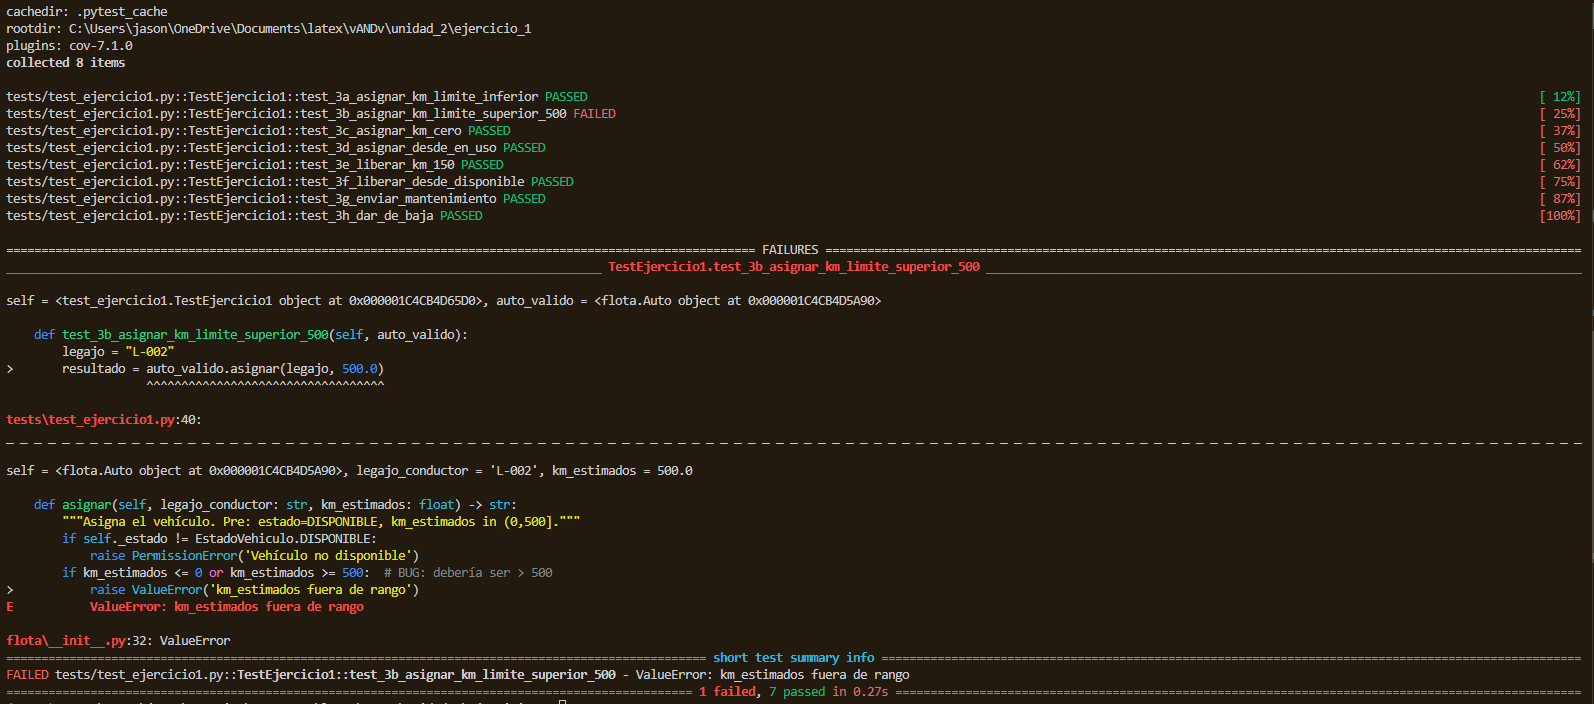
\includegraphics[width=0.8\textwidth]{ima1.png}
    \caption{Resultado del test 3.c en pytest. Se observa que se lanza la excepción esperada y el estado del vehículo no cambia.}
    \label{fig:diagrama-estados-auto}
\end{figure}

\subsection{Consigna 4: Verificación del invariante tras excepciones}

Para cada caso que espera una excepción (3.c, 3.d, 3.f), se incluyó un assert adicional que verifica que el estado del objeto no cambió tras la excepción:

\begin{itemize}
    \item \textbf{3.c:} Tras \texttt{ValueError} por km=0.0, el estado permanece DISPONIBLE y los km no varían.
    \item \textbf{3.d:} Tras \texttt{PermissionError} por estado EN\_USO, el estado se mantiene en EN\_USO y los km no cambian.
    \item \textbf{3.f:} Tras \texttt{PermissionError} por estado DISPONIBLE, el estado permanece DISPONIBLE y los km no cambian.
\end{itemize}

\subsection{Consigna 5: Medición de cobertura}

Se ejecutó \texttt{pytest --cov --branch} para medir la cobertura. Los resultados obtenidos son:


\begin{figure}[ht]
    \centering
    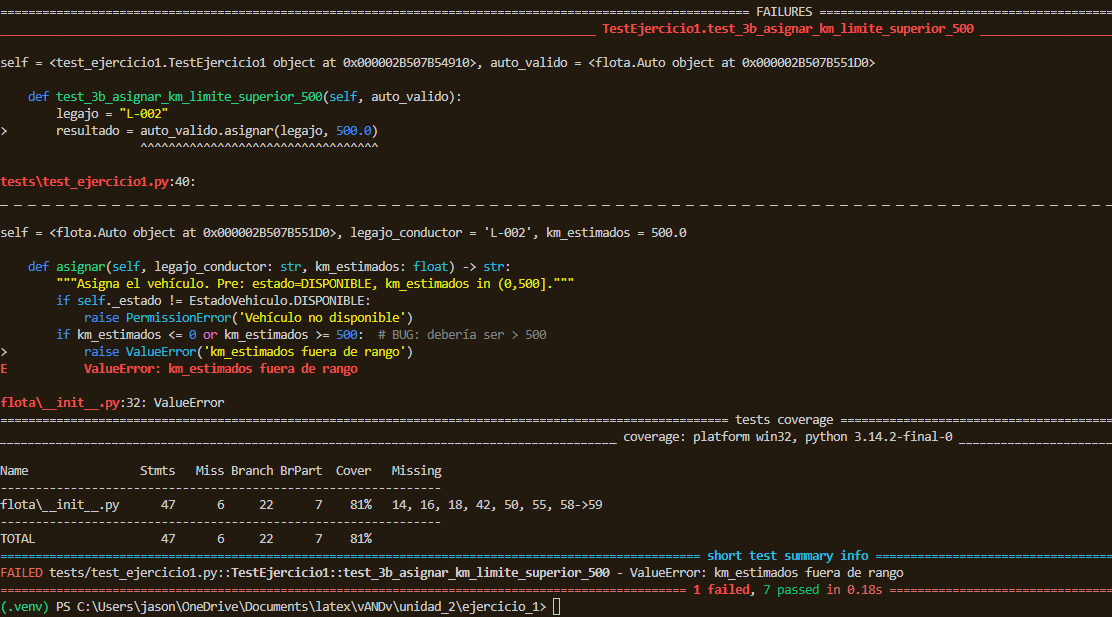
\includegraphics[width=0.8\textwidth]{ima2.png}
    \caption{Resultado de aplicar -v --cov=flota --cov-branch a los tests de \texttt{auto.py}. Se observa que se alcanzó un C0 del 87,23\% y un C1 del 63,64\%.}
    \label{fig:diagrama-estados-auto}
\end{figure}


Con ayuda de la Unidad N° 1 (definición 4.2 y 4.3) sabemos que C0 toda sentencia del programa es ejectuada por al menos un caso de prueba (sentencias ejecutadas/total sentencia)*100%. Todo arco del GFC es recorrido por al menos un caso de prueba (arcos ejercitados / total arcos)*100%. En este caso, se obtuvo un C0 del 87,23\% y un C1 del 63,64\%, lo que indica que la mayoría de las sentencias fueron ejecutadas por los tests, pero hay ramas de código (condicionales) que no fueron completamente cubiertas por los casos de prueba implementados. Esto se debe a que algunos escenarios de error no fueron testeados, como se detalla a continuación.


\begin{table}[ht]
\centering
\caption{Resultados de cobertura --- \texttt{auto.py}}
\label{tab:cobertura-auto}
\begin{tabular}{lcc}
\toprule
Métrica & Valor & \\
\midrule
Sentencias totales (Stmts) & 47 & \\
Sentencias ejecutadas & 41 & \\
Sentencias no ejecutadas (Miss) & 6 & \\
\textbf{C0 (cobertura de sentencias)} & \textbf{87,23\%} & $(41/47 \times 100)$ \\
\textbf{C1 (cobertura de ramas)} & \textbf{63,64\%} & $(8/22 \times 100)$ \\
\midrule
Ramas totales & 22 & \\
Ramas no cubiertas & 8 & \\
Ramas parciales & 7 & \\
\bottomrule
\end{tabular}
\end{table}

\subsubsection*{Ramas no cubiertas}

\begin{table}[ht]
\centering
\caption{Sentencias no cubiertas en \texttt{auto.py}}
\label{tab:no-cubiertas-auto}
\begin{tabular}{cp{6cm}p{4cm}}
\toprule
Línea & Sentencia & Razón \\
\midrule
12 & \texttt{raise ValueError('Patente inválida')} & No se testeó con patente vacía o len $<$ 6 \\
14 & \texttt{raise ValueError('km\_actuales $<$ 0')} & No se testeó con km\_actuales $<$ 0 \\
16 & \texttt{raise ValueError('num\_puertas debe ser 2, 4 o 5')} & No se testeó con num\_puertas $\notin \{2,4,5\}$ \\
42 & \texttt{raise ValueError('km\_recorridos $<$ 0')} & No se testeó \texttt{liberar()} con km\_recorridos $<$ 0 \\
51 & \texttt{raise PermissionError('...mantenimiento en uso')} & No se testeó \texttt{enviar\_mantenimiento()} desde EN\_USO \\
57 & \texttt{raise PermissionError('...baja...en uso')} & No se testeó \texttt{dar\_de\_baja()} desde EN\_USO \\
\bottomrule
\end{tabular}
\end{table}

Las ramas parciales (líneas 11, 13, 15, 41, 50, 56, 61) corresponden a condiciones donde solo se ejecutó la rama \texttt{False} (la condición no se cumplió), pero nunca la rama \texttt{True}. Por ejemplo, en la línea 11 \texttt{if not patente or len(patente) < 6}, siempre se pasó una patente válida, por lo que la rama que lanza la excepción nunca se tomó.


Los tests implementados cubren los caminos principales de cada método y los casos de error especificados en las consignas, logrando un C0 de 87,23\%. El C1 de 63,64\% indica que hay ramas de validación de entrada en el constructor y de métodos que no fueron ejercitadas porque los casos de prueba se centraron en los escenarios de asignación/liberación y transiciones de estado definidos en la consigna.

\FloatBarrier
% ============================================================
% EJERCICIO 2
% ============================================================
\section{FSM y Testing basado en Estado --- Vehiculo de Flota}

\subsection{Consigna 6: Tabla de transición (Algoritmo 2.2)}

Aplicamos el \textbf{Algoritmo 2.2} paso a paso:

\textbf{Paso 1.} Identificar los estados. Según la especificación verbal y la Definición 2.6, los estados son los grupos de valores de atributos que producen comportamientos cualitativamente distintos:
\[
S = \{\text{DISPONIBLE}, \text{EN\_USO}, \text{MANTENIMIENTO}, \text{BAJA}\}
\]

\textbf{Paso 2.} Identificar el estado inicial. El objeto queda en \texttt{DISPONIBLE} inmediatamente después del constructor:
\[
s_0 = \text{DISPONIBLE}
\]

\textbf{Paso 3.} Para cada método público y cada estado, determinar si es aplicable. Los eventos (métodos que modifican el estado) son:
\[
\Sigma = \{\text{asignar()}, \text{liberar()}, \text{enviarMantenimiento()}, \text{darDeBaja()}\}
\]


\begin{figure}[ht]
    \centering
    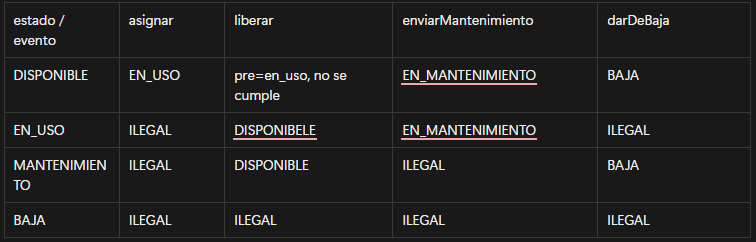
\includegraphics[width=0.8\textwidth]{ima3.png}
    \caption{Tabla de transición de la FSM para Vehiculo (Algoritmo 2.2). Cada celda indica el estado destino y efecto si la transición es válida, o la excepción si no lo es.}
    \label{fig:diagrama-estados-auto}
\end{figure}



\textbf{Justificación de cada celda según la especificación:}

\begin{itemize}
    \item \textbf{DISPONIBLE + asignar():} Válida. El vehículo puede ser asignado a un conductor. Transición DISPONIBLE $\rightarrow$ EN\_USO.
    \item \textbf{DISPONIBLE + liberar():} Inválida. No se puede liberar un vehículo que no está en uso. Lanza \texttt{PermissionError}.
    \item \textbf{DISPONIBLE + enviarMantenimiento():} Válida. Se puede enviar a mantenimiento preventivo. Transición DISPONIBLE $\rightarrow$ MANTENIMIENTO.
    \item \textbf{DISPONIBLE + darDeBaja():} Válida. Se puede dar de baja desde cualquier estado excepto EN\_USO. Transición DISPONIBLE $\rightarrow$ BAJA.
    \item \textbf{EN\_USO + asignar():} Inválida. Ya está asignado. Lanza \texttt{PermissionError}.
    \item \textbf{EN\_USO + liberar():} Válida. Finaliza el viaje. Transición EN\_USO $\rightarrow$ DISPONIBLE.
    \item \textbf{EN\_USO + enviarMantenimiento():} Válida. Mantenimiento correctivo por avería. Transición EN\_USO $\rightarrow$ MANTENIMIENTO.
    \item \textbf{EN\_USO + darDeBaja():} Inválida. No se puede dar de baja un vehículo en uso. Lanza \texttt{PermissionError}.
    \item \textbf{MANTENIMIENTO + asignar():} Inválida. Está en el taller. Lanza \texttt{PermissionError}.
    \item \textbf{MANTENIMIENTO + liberar():} Válida. Finaliza la revisión y vuelve a disponible. Transición MANTENIMIENTO $\rightarrow$ DISPONIBLE.
    \item \textbf{MANTENIMIENTO + enviarMantenimiento():} Inválida. Ya está en mantenimiento. Lanza \texttt{PermissionError}.
    \item \textbf{MANTENIMIENTO + darDeBaja():} Válida. Se puede dar de baja desde mantenimiento. Transición MANTENIMIENTO $\rightarrow$ BAJA.
    \item \textbf{BAJA + cualquier operación:} Todas inválidas. El vehículo fue retirado definitivamente. Lanza \texttt{IllegalStateException}.
\end{itemize}

\subsection{Consigna 7: Diagrama de estados UML}

Se construye a partir de la tabla de transición.

\begin{figure}[ht]
\centering
\begin{tikzpicture}[
    state/.style={rectangle, rounded corners, draw=black, thick, minimum width=2.5cm, minimum height=1cm, align=center},
    initial/.style={circle, fill=black, minimum size=0.4cm, inner sep=0pt},
    arrow/.style={-Stealth, thick}
]
% Estados
\node[initial] (init) {};
\node[state, right=1.2cm of init] (disponible) {DISPONIBLE};
\node[state, right=3cm of disponible] (enUso) {EN\_USO};
\node[state, below=2cm of disponible] (mantenimiento) {MANTENIMIENTO};
\node[state, below=2cm of enUso] (baja) {BAJA};

% Nodo inicial -> DISPONIBLE
\draw[arrow] (init) -- (disponible);

% Transiciones válidas
\draw[arrow] (disponible) -- node[above, font=\small] {asignar()} (enUso);
\draw[arrow] (enUso) -- node[below, font=\small] {liberar()} (disponible);
\draw[arrow] (disponible) -- node[left, font=\small] {enviarMant.} (mantenimiento);
\draw[arrow] (enUso) -- node[right, font=\small] {enviarMant.} (mantenimiento);
\draw[arrow] (mantenimiento) -- node[left, font=\small] {liberar()} (disponible);
\draw[arrow] (disponible) -- node[above right, font=\scriptsize] {darDeBaja()} (baja);
\draw[arrow] (mantenimiento) -- node[below, font=\small] {darDeBaja()} (baja);

% Transiciones inválidas (con rayas)
\draw[arrow, dashed, red] (disponible) -- node[below left, font=\scriptsize, red] {liberar() $\times$} ++(-0.5, -0.8);
\draw[arrow, dashed, red] (enUso) -- node[above, font=\scriptsize, red] {asignar() $\times$} ++(0, 1.2);
\draw[arrow, dashed, red] (enUso) -- node[below right, font=\scriptsize, red] {darDeBaja() $\times$} ++(0.5, -0.8);
\draw[arrow, dashed, red] (mantenimiento) -- node[above, font=\scriptsize, red] {asignar() $\times$} ++(-0.5, 0.8);
\draw[arrow, dashed, red] (mantenimiento) -- node[below, font=\scriptsize, red] {enviarMant() $\times$} ++(0.5, -0.8);
\draw[arrow, dashed, red] (baja) -- node[below, font=\scriptsize, red] {todas $\times$} ++(1.5, 0);

\end{tikzpicture}
\caption{Diagrama de estados para Vehiculo. Flechas sólidas: transiciones válidas. Flechas punteadas rojas: transiciones inválidas (excepción).}
\label{fig:diagrama-estados}
\end{figure}

\textbf{Elementos del diagrama:}
\begin{itemize}
    \item \textbf{Nodo inicial:} Círculo negro apuntando a DISPONIBLE, indicando que es el estado tras la construcción del objeto.
    \item \textbf{Estados:} Rectángulos para cada estado de la FSM.
    \item \textbf{Transiciones válidas:} Flechas etiquetadas con el evento (método) que las dispara.
    \item \textbf{Transiciones inválidas:} Flechas punteadas indicando que la operación lanza excepción y el estado no cambia.
    \item \textbf BAJA es un estado que no tiene transiciones salientes válidas.
\end{itemize}

\subsection{Consigna 8: Casos de prueba C-Trans (Algoritmo 2.3) en JUnit 5}

\noindent Código fuente (clases del dominio): \href{https://github.com/Cristopher-Ovaillos/Unidad_2_ValidacionVerificacion/tree/main/Unidad_2_code/ejercicio_2/src/main/java/com/example/}{\texttt{ejercicio\_2/src/main/java/}} \\
Tests: \href{https://github.com/Cristopher-Ovaillos/Unidad_2_ValidacionVerificacion/blob/main/Unidad_2_code/ejercicio_2/src/test/java/com/example/Ejercicio2Test.java}{\texttt{Ejercicio2Test.java}} y \href{https://github.com/Cristopher-Ovaillos/Unidad_2_ValidacionVerificacion/blob/main/Unidad_2_code/ejercicio_2/src/test/java/com/example/Ejercicio3LspTest.java}{\texttt{Ejercicio3LspTest.java}}

Aplicamos el \textbf{Algoritmo 2.3} paso a paso:

\textbf{Paso 1.} La FSM y su tabla de transición ya fueron construidas (Consigna 6).

\textbf{Paso 2.} Listar todas las transiciones válidas y marcarlas como NO CUBIERTAS:

\begin{itemize}
    \item \textbf{T1:} DISPONIBLE $\rightarrow$ EN\_USO \hfill \texttt{asignar()}
    \item \textbf{T2:} DISPONIBLE $\rightarrow$ MANTENIMIENTO \hfill \texttt{enviarMantenimiento()}
    \item \textbf{T3:} DISPONIBLE $\rightarrow$ BAJA \hfill \texttt{darDeBaja()}
    \item \textbf{T4:} EN\_USO $\rightarrow$ DISPONIBLE \hfill \texttt{liberar()}
    \item \textbf{T5:} EN\_USO $\rightarrow$ MANTENIMIENTO \hfill \texttt{enviarMantenimiento()}
    \item \textbf{T6:} MANTENIMIENTO $\rightarrow$ DISPONIBLE \hfill \texttt{liberar()}
    \item \textbf{T7:} MANTENIMIENTO $\rightarrow$ BAJA \hfill \texttt{darDeBaja()}
\end{itemize}

Son \textbf{7 transiciones válidas} en total.

\textbf{Paso 3.} Para cada transición, diseñar la secuencia que lleve al objeto desde $s_0$ hasta el estado origen:

\begin{itemize}
    \item \textbf{T1, T2, T3:} El estado origen es DISPONIBLE, que es el estado inicial $s_0$. No se necesita secuencia previa; basta con \texttt{new Vehiculo()}.
    \item \textbf{T4, T5:} El estado origen es EN\_USO. Secuencia: \texttt{new Vehiculo()} $\rightarrow$ \texttt{asignar()}.
    \item \textbf{T6, T7:} El estado origen es MANTENIMIENTO. Secuencia: \texttt{new Vehiculo()} $\rightarrow$ \texttt{enviarMantenimiento()} (desde DISPONIBLE).
\end{itemize}

\textbf{Paso 4-6.} Implementación completa en JUnit 5:

\begin{lstlisting}[language=Java, caption={TestVehiculoTransiciones.java --- Cobertura C-Trans completa}]
import static org.junit.jupiter.api.Assertions.*;
import org.junit.jupiter.api.BeforeEach;
import org.junit.jupiter.api.Test;

class TestVehiculoTransiciones {

    private Vehiculo vehiculo;

    @BeforeEach
    void setUp() {
        //cada test comienza con un vehiculo nuevo en DISPONIBLE
        vehiculo = new Vehiculo("ABC123", "Toyota", 2020);
        assertEquals(EstadoVehiculo.DISPONIBLE, vehiculo.getEstado());
    }

    // trans. validas

    //T1
    @Test
    void asignar_desde_disponible_cambia_a_en_uso() {
        //DISPONIBLE- a EN_USO via asignar(legajo, km)
        //ARRANGE: vehiculo ya esta en DISPONIBLE
        String legajo = "L-001";
        double kmEstimados = 100.0;
        //ACT
        String resultado = vehiculo.asignar(legajo, kmEstimados);
        //ASSERT: estado destino + efecto + invariante
        assertEquals(EstadoVehiculo.EN_USO, vehiculo.getEstado());
        assertNotNull(resultado);
        assertTrue(resultado.contains(legajo));
        assertTrue(vehiculo.getKm() >= 0); // invariante
    }

    //T2
    @Test
    void enviarMantenimiento_desde_disponible_cambia_a_mantenimiento() {
        //DISPONIBLE -> MANTENIMIENTO  enviarMantenimiento()
        //ARRANGE: vehiculo ya esta en DISPONIBLE (setUp)
        // ACT
        vehiculo.enviarMantenimiento();
        // ASSERT
        assertEquals(EstadoVehiculo.MANTENIMIENTO, vehiculo.getEstado());
        assertTrue(vehiculo.getKm() >= 0); // invariante
    }

    //T3
    @Test
    void darDeBaja_desde_disponible_cambia_a_baja() {
        //DISPONIBLE -> BAJA darDeBaja()
        //ARRANGE: vehiculo ya esta en DISPONIBLE 
        //ACT
        vehiculo.darDeBaja();
        //ASSERT
        assertEquals(EstadoVehiculo.BAJA, vehiculo.getEstado());
        assertTrue(vehiculo.getKm() >= 0); // invariante
    }

    //T4
    @Test
    void liberar_desde_en_uso_cambia_a_disponible() {
        //EN_USO -> DISPONIBLE via liberar(kmRec)
        //ARRANGE: llevar a EN_USO
        vehiculo.asignar("L-002", 200.0);
        assertEquals(EstadoVehiculo.EN_USO, vehiculo.getEstado());
        double kmAntes = vehiculo.getKm();

        // ACT
        vehiculo.liberar(150.0);

        // ASSERT: estado destino + efecto + invariante
        assertEquals(EstadoVehiculo.DISPONIBLE, vehiculo.getEstado());
        assertEquals(kmAntes + 150.0, vehiculo.getKm(), 0.001);
        assertTrue(vehiculo.getKm() >= 0); // invariante
    }

    //T5
    @Test
    void enviarMantenimiento_desde_en_uso_cambia_a_mantenimiento() {
        //EN_USO -> MANTENIMIENTO via enviarMantenimiento()
        //ARRANGE: llevar a EN_USO
        vehiculo.asignar("L-003", 50.0);
        assertEquals(EstadoVehiculo.EN_USO, vehiculo.getEstado());

        // ACT
        vehiculo.enviarMantenimiento();

        // ASSERT
        assertEquals(EstadoVehiculo.MANTENIMIENTO, vehiculo.getEstado());
        assertTrue(vehiculo.getKm() >= 0); // invariante
    }

    //T6
    @Test
    void liberar_desde_mantenimiento_cambia_a_disponible() {
        //MANTENIMIENTO -> DISPONIBLE  liberar(kmRec)
        //ARRANGE: llevar a MANTENIMIENTO
        vehiculo.enviarMantenimiento();
        assertEquals(EstadoVehiculo.MANTENIMIENTO, vehiculo.getEstado());
        double kmAntes = vehiculo.getKm();

        // ACT
        vehiculo.liberar(0.0);

        // ASSERT
        assertEquals(EstadoVehiculo.DISPONIBLE, vehiculo.getEstado());
        assertEquals(kmAntes, vehiculo.getKm(), 0.001); // no se suman km
        assertTrue(vehiculo.getKm() >= 0); // invariante
    }

    //T7
    @Test
    void darDeBaja_desde_mantenimiento_cambia_a_baja() {
        //MANTENIMIENTO -> BAJA via darDeBaja()
        //ARRANGE: llevar a MANTENIMIENTO
        vehiculo.enviarMantenimiento();
        assertEquals(EstadoVehiculo.MANTENIMIENTO, vehiculo.getEstado());

        // ACT
        vehiculo.darDeBaja();

        // ASSERT
        assertEquals(EstadoVehiculo.BAJA, vehiculo.getEstado());
        assertTrue(vehiculo.getKm() >= 0); // invariante
    }
}
\end{lstlisting}

\subsection{Consigna 9: Transiciones inválidas}

Para todas las transiciones inválidas de la tabla. Según el Algoritmo 2.3, Paso 5: para cada celda con excepción, verificar que se lanza la excepción correcta y que el estado del objeto no cambia.

Las transiciones inválidas son:

\begin{itemize}
    \item \textbf{INV1:} DISPONIBLE + \texttt{liberar()} $\rightarrow$ \texttt{PermissionError}
    \item \textbf{INV2:} EN\_USO + \texttt{asignar()} $\rightarrow$ \texttt{PermissionError}
    \item \textbf{INV3:} EN\_USO + \texttt{darDeBaja()} $\rightarrow$ \texttt{PermissionError}
    \item \textbf{INV4:} MANTENIMIENTO + \texttt{asignar()} $\rightarrow$ \texttt{PermissionError}
    \item \textbf{INV5:} MANTENIMIENTO + \texttt{enviarMantenimiento()} $\rightarrow$ \texttt{PermissionError}
    \item \textbf{INV6:} BAJA + \texttt{asignar()} $\rightarrow$ \texttt{IllegalStateException}
    \item \textbf{INV7:} BAJA + \texttt{liberar()} $\rightarrow$ \texttt{IllegalStateException}
    \item \textbf{INV8:} BAJA + \texttt{enviarMantenimiento()} $\rightarrow$ \texttt{IllegalStateException}
    \item \textbf{INV9:} BAJA + \texttt{darDeBaja()} $\rightarrow$ \texttt{IllegalStateException}
\end{itemize}

Son \textbf{9 transiciones inválidas} en total.

\begin{lstlisting}[language=Java, caption={TestVehiculoTransicionesInvalidas.java}]
class TestVehiculoTransicionesInvalidas {

    private Vehiculo vehiculo;

    @BeforeEach
    void setUp() {
        vehiculo = new Vehiculo("ABC123", "Toyota", 2020);
    }

    //INV1
    @Test
    void liberar_desde_disponible_lanza_permission_error() {
        //DISPONIBLE
        EstadoVehiculo estadoInicial = vehiculo.getEstado();
        double kmInicial = vehiculo.getKm();
        assertEquals(EstadoVehiculo.DISPONIBLE, estadoInicial);

        assertThrows(PermissionError.class,
            () -> vehiculo.liberar(100.0));

        // Verificar que el estado no cambio
        assertEquals(estadoInicial, vehiculo.getEstado());
        assertEquals(kmInicial, vehiculo.getKm(), 0.001);
        assertTrue(vehiculo.getKm() >= 0); // invariante
    }

    //INV2
    @Test
    void asignar_desde_en_uso_lanza_permission_error() {
        vehiculo.asignar("L-010", 100.0);
        EstadoVehiculo estadoInicial = vehiculo.getEstado();
        double kmInicial = vehiculo.getKm();
        assertEquals(EstadoVehiculo.EN_USO, estadoInicial);

        assertThrows(PermissionError.class,
            () -> vehiculo.asignar("L-011", 50.0));

        assertEquals(estadoInicial, vehiculo.getEstado());
        assertEquals(kmInicial, vehiculo.getKm(), 0.001);
        assertTrue(vehiculo.getKm() >= 0); // invariante
    }

    //INV3
    @Test
    void darDeBaja_desde_en_uso_lanza_permission_error() {
        vehiculo.asignar("L-012", 100.0);
        EstadoVehiculo estadoInicial = vehiculo.getEstado();
        assertEquals(EstadoVehiculo.EN_USO, estadoInicial);

        assertThrows(PermissionError.class,
            () -> vehiculo.darDeBaja());

        assertEquals(estadoInicial, vehiculo.getEstado());
        assertTrue(vehiculo.getKm() >= 0); // invariante
    }

    //INV4
    @Test
    void asignar_desde_mantenimiento_lanza_permission_error() {
        vehiculo.enviarMantenimiento();
        EstadoVehiculo estadoInicial = vehiculo.getEstado();
        assertEquals(EstadoVehiculo.MANTENIMIENTO, estadoInicial);

        assertThrows(PermissionError.class,
            () -> vehiculo.asignar("L-013", 50.0));

        assertEquals(estadoInicial, vehiculo.getEstado());
        assertTrue(vehiculo.getKm() >= 0); // invariante
    }

    //INV5
    @Test
    void enviarMantenimiento_desde_mantenimiento_lanza_permission_error() {
        vehiculo.enviarMantenimiento();
        EstadoVehiculo estadoInicial = vehiculo.getEstado();
        assertEquals(EstadoVehiculo.MANTENIMIENTO, estadoInicial);

        assertThrows(PermissionError.class,
            () -> vehiculo.enviarMantenimiento());

        assertEquals(estadoInicial, vehiculo.getEstado());
        assertTrue(vehiculo.getKm() >= 0); // invariante
    }

    // Helper para llevar a BAJA
    private void llevarABaja() {
        vehiculo.enviarMantenimiento(); // DISPONIBLE -> MANTENIMIENTO
        vehiculo.darDeBaja();           // MANTENIMIENTO -> BAJA
    }

    //INV6
    @Test
    void asignar_desde_baja_lanza_illegal_state() {
        llevarABaja();
        EstadoVehiculo estadoInicial = vehiculo.getEstado();
        assertEquals(EstadoVehiculo.BAJA, estadoInicial);

        assertThrows(IllegalStateException.class,
            () -> vehiculo.asignar("L-014", 50.0));

        assertEquals(estadoInicial, vehiculo.getEstado());
    }

    //INV7
    @Test
    void liberar_desde_baja_lanza_illegal_state() {
        llevarABaja();
        EstadoVehiculo estadoInicial = vehiculo.getEstado();
        assertEquals(EstadoVehiculo.BAJA, estadoInicial);

        assertThrows(IllegalStateException.class,
            () -> vehiculo.liberar(100.0));

        assertEquals(estadoInicial, vehiculo.getEstado());
    }

    //INV8
    @Test
    void enviarMantenimiento_desde_baja_lanza_illegal_state() {
        llevarABaja();
        EstadoVehiculo estadoInicial = vehiculo.getEstado();
        assertEquals(EstadoVehiculo.BAJA, estadoInicial);

        assertThrows(IllegalStateException.class,
            () -> vehiculo.enviarMantenimiento());

        assertEquals(estadoInicial, vehiculo.getEstado());
    }

    //INV9
    @Test
    void darDeBaja_desde_baja_lanza_illegal_state() {
        llevarABaja();
        EstadoVehiculo estadoInicial = vehiculo.getEstado();
        assertEquals(EstadoVehiculo.BAJA, estadoInicial);

        assertThrows(IllegalStateException.class,
            () -> vehiculo.darDeBaja());

        assertEquals(estadoInicial, vehiculo.getEstado());
    }
}
\end{lstlisting}


\begin{enumerate}
    \item \textbf{Arrange:} Preparar el objeto en el estado origen requerido.
    \item con variables temp guardar el estado y atributos antes de invocar la operación inválida.
    \item \textbf{Act + Assert:} Usar \texttt{assertThrows} para verificar que se lanza la excepción esperada.
    \item Confirmar que el estado y los atributos no cambiaron tras la excepción (el invariante se preserva).
\end{enumerate}

Según el Algoritmo 2.3, Paso 6: ``Verificar que el invariante se cumple en todos los casos, incluyendo los de excepción.''

\subsection{Consigna 10: Cálculo de casos}

\textbf{(a) Número mínimo de casos para C-Trans:}

Según la Propiedad 2.2 del apunte, la cobertura C-Trans requiere que toda transición válida de la FSM sea ejercitada por al menos un caso. Contando las transiciones válidas de la tabla (Consigna 6):

\[
\text{C-Trans mínimo} = |T_{válidas}| = 7 \text{ casos}
\]

Cada transición válida necesita al menos un caso de prueba, y en este diseño cada caso ejercita exactamente una transición, por lo que \textbf{7} es el mínimo.

\textbf{(b) Número de casos adicionales para transiciones inválidas:}

Las transiciones inválidas son las celdas de la tabla que contienen excepciones:

\[
\text{Inválidas} = 16 \text{ celdas totales} - 7 \text{ válidas} = 9 \text{ casos adicionales}
\]

Se necesitan \textbf{9 casos adicionales}, uno por cada combinación (estado, método) que lanza excepción.

\textbf{(c) Casos adicionales para C-Par en la secuencia DISPONIBLE $\rightarrow$ EN\_USO $\rightarrow$ MANTENIMIENTO:}

La cobertura C-Par (Definición 2.9) requiere que todo par de transiciones consecutivas sea ejercitado. La secuencia DISPONIBLE $\rightarrow$ EN\_USO $\rightarrow$ MANTENIMIENTO involucra el par:
\[
(\text{DISPONIBLE} \xrightarrow{\text{asignar()}} \text{EN\_USO}, \quad \text{EN\_USO} \xrightarrow{\text{enviarMantenimiento()}} \text{MANTENIMIENTO})
\]

Este par ya está parcialmente cubierto por los tests individuales T1 y T5, pero C-Par exige que ambas transiciones se ejecuten \textbf{consecutivamente} en un solo caso de prueba para verificar que el comportamiento después de la primera transición no afecta a la segunda.

El test T5 ya lleva el vehículo a EN\_USO y luego invoca \texttt{enviarMantenimiento()}, pero lo hace en un solo test. Sin embargo, T5 no verifica explícitamente el estado intermedio EN\_USO como punto de verificación antes de la segunda transición. Para C-Par estricto se necesita un caso adicional que:

\begin{enumerate}
    \item Parta de DISPONIBLE.
    \item Ejecute \texttt{asignar()} y verifique EN\_USO.
    \item Ejecute \texttt{enviarMantenimiento()} y verifique MANTENIMIENTO.
    \item Verifique el invariante tras cada transición.
\end{enumerate}

Si bien T5 ya ejecuta esta secuencia, un caso de C-Par explícito añadiría asserts intermedios. Por lo tanto, \textbf{se necesita 1 caso adicional} para C-Par estricto de esta secuencia específica.

\begin{lstlisting}[language=Java, caption={Caso adicional para C-Par: DISPONIBLE \(\to\) EN\_USO \(\to\) MANTENIMIENTO}]
@Test
void cpar_disponible_en_uso_mantenimiento() {
    // Par de transiciones consecutivas:
    // (DISPONIBLE -> EN_USO, EN_USO -> MANTENIMIENTO)

    // Paso 1: DISPONIBLE -> EN_USO
    assertEquals(EstadoVehiculo.DISPONIBLE, vehiculo.getEstado());
    vehiculo.asignar("L-020", 100.0);
    assertEquals(EstadoVehiculo.EN_USO, vehiculo.getEstado());
    assertTrue(vehiculo.getKm() >= 0); // invariante tras 1ra transicion

    // Paso 2: EN_USO -> MANTENIMIENTO
    vehiculo.enviarMantenimiento();
    assertEquals(EstadoVehiculo.MANTENIMIENTO, vehiculo.getEstado());
    assertTrue(vehiculo.getKm() >= 0); // invariante tras 2da transicion
}
\end{lstlisting}


La jerarquía de coberturas establece que C-Estado $\subset$ C-Trans $\subset$ C-Par (Propiedad 2.2). C-Trans es el criterio mínimo recomendado y ya garantiza C-Estado. C-Par es más fuerte y detecta defectos de interacción entre métodos consecutivos que C-Trans no alcanza.

\FloatBarrier




\section{Testing Polimórfico y LSP — jerarquía Vehiculo}

\subsection{Consigna 11: Implementá la Suite Heredada (Definición 2.11) como clase abstracta de test en Java. Debe contener un caso de prueba por cada combinación método × clase de equivalencia del contrato de la superclase.}

En este ejercicio debemos identificar las clases de equivalencias con ayuda del temario de la Unidad I y el algoritmo 2.4 (Verificacíon de LSP).

El algoritmo 2.4 presente los siguientes pasos:

\begin{itemize}
    \item Paso 1: identificar la superclase (Vehiculo) y subclases (Auto, Camion, Moto).
    \item Paso 2: Para la superclase documetnar el contrato de cada metodo publico (pre, post, invariante) \ref{fig:contrato_vehiculo}.
    \item Paso 3: Construir la suite heredada, un caso de prueba por cada combinacion metodo por clase de dequivalencia de entrada (\ref{tab:ce_asignar})
\end{itemize}



\begin{figure}[ht]
    \centering
    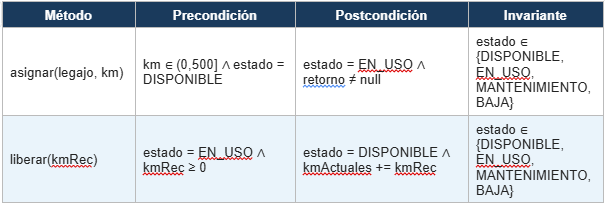
\includegraphics[width=0.8\textwidth]{contrato_tp.png}
    \caption{Contrato de cada metodo de Vehiculo.}
    \label{fig:contrato_vehiculo}
\end{figure}

Para identificar las clases de equivalencia aplicaremos el algoritmo 1.6 sobre el contrato de la superclase (separado por metodo).

\begin{table}[ht]
    \centering
    \caption{clases de equivalencia - Vehiculo.asignar(legajo, km)}
    \label{tab:ce_asignar}
    \begin{tabular}{lllll} % 'l' significa alineado a la izquierda (left)
        \toprule
        \textbf{Variable} & \textbf{Clase} & \textbf{Condición} & \textbf{tipo} & \textbf{Rep} \\
        \midrule
        legajo(R1)   & CE1   & 0<km<=500 & valida & 100\\
        legajo(R1)   & CE2   & km<=0 & no valida & 0\\
        legajo(R1)   & CE3   & km>500 & no valida & 501\\
        estado(R3)   & CE4   & estado==disponible & valida & DISPONIBLE\\
        estado(R3)   & CE5   & estado!=disponible & no valida & estado in \{EN\_USO, MANTENIMIENTO, BAJA\}\\
        \bottomrule
    \end{tabular}
\end{table}




Diseño de la suite heredada

Segun la definicion 2.11 y paso 3, construimos un caso de prueba por cada combinacion metodo x clase de equivalencia del contrato.

Para cada metodo, identificamos sus entraas y estados posibles, y las dividimos en particiones validas e invalidas y luego un test que use un representante de cada clase de equivalencia y ejecutar el metodo bajo esas condiciones. 

\begin{table}[ht]
    \centering
    \caption{Casos de prueba - Vehiculo.asignar() y Vehiculo.liberar()}
    \label{tab:casos_prueba}
    \begin{tabular}{|c|l|l|l|l|}
        \hline
        ID & Método & Combinación de CE & Representantes & Resultado Esperado \\ 
        \hline
        
        TC1 & asignar & CE1 (V) + CE4 (V) & km: 100, estado: DISPONIBLE & Éxito: estado pasa a EN\_USO \\ 
        \hline
        
        TC2 & asignar & CE2 (I) + CE4 (V) & km: 0, estado: DISPONIBLE & Error: IllegalArgumentException \\ 
        \hline
        
        TC3 & asignar & CE3 (I) + CE4 (V) & km: 501, estado: DISPONIBLE & Error: IllegalArgumentException \\ 
        \hline
        
        TC4 & asignar & CE1 (V) + CE5 (I) & km: 100, estado: EN\_USO & Error: IllegalStateException \\ 
        \hline
        
        TC5 & liberar & CE6 (V) + CE8 (V) & estado: EN\_USO, kmRec: 150 & Éxito: estado pasa a DISPONIBLE \\ 
        \hline
        
        TC6 & liberar & CE7 (I) + CE8 (V) & estado: DISPONIBLE, kmRec: 150 & Error: IllegalStateException \\ 
        \hline
        
        TC7 & liberar & CE6 (V) + CE9 (I) & estado: EN\_USO, kmRec: -10 & Error: IllegalArgumentException \\ 
        \hline
        
    \end{tabular}
\end{table}



\subsection{Consigna 12: Aplicá el Algoritmo 2.4: ejecutá la Suite Heredada sobre cada subclase concreta (Auto, Moto, Camion) sustituyendo instancias.}

\begin{itemize}
    \item Paso 4: Para cada subclase, ejecutar la suite heredada usando instancias de subclase donde se esperaban instancias de C.
\end{itemize}


Este paso consiste en realizar sustitucion de instancias, totmamos la suite heredada (es decir, la clase abstracta del ejercicio 11) y la conectamos con los objetos instanciados de Auto, Moto, Camion. Recordar que \textbf{Vehiculo v= new Auto()}, en tiempo de compilacion este es de tipo Vehiculo, en ejecución es de tipo Auto.

En JUNIT, se logra creando una clase de test para cada subclase de vehiculo que extendera de la clase abstracta. Asi, los mismos test del contrato padre se ejecutan automaticamente sobre cada hijo.
Cada subclase implemente el metodo \textbf{crearVehiculo} devolviendo su propio tipo de objeto.

Código fuente (clases del dominio): \href{https://github.com/Cristopher-Ovaillos/Unidad_2_ValidacionVerificacion/tree/main/Unidad_2_code/ejercicio_3/auto/src/main/java/com/enunciado_3/}{\texttt{ejercicio\_3/auto/src/main/java/}} \\
Suite Heredada (test abstracto): \href{https://github.com/Cristopher-Ovaillos/Unidad_2_ValidacionVerificacion/blob/main/Unidad_2_code/ejercicio_3/auto/src/test/java/com/enunciado_3/VehiculoTest.java}{\texttt{VehiculoTest.java}} \\
Tests por subclase: \href{https://github.com/Cristopher-Ovaillos/Unidad_2_ValidacionVerificacion/blob/main/Unidad_2_code/ejercicio_3/auto/src/test/java/com/enunciado_3/AutoTest.java}{\texttt{AutoTest.java}}, \href{https://github.com/Cristopher-Ovaillos/Unidad_2_ValidacionVerificacion/blob/main/Unidad_2_code/ejercicio_3/auto/src/test/java/com/enunciado_3/MotoTest.java}{\texttt{MotoTest.java}}, \href{https://github.com/Cristopher-Ovaillos/Unidad_2_ValidacionVerificacion/blob/main/Unidad_2_code/ejercicio_3/auto/src/test/java/com/enunciado_3/CamionTest.java}{\texttt{CamionTest.java}}

Con esto verificremos el cumplimiento del principio de sustitución de Liskov de manera dinamica, es decir, mediante la ejecución de los test de las subclases.

Esto utiliza herencia de clases de test. La clase test abstracta de vehiculo es el contrato y las nuevas clases clases que herendan esta realizal la sustitución de instancia.
La suite abstracta llama a \textbf{crearVehiculo()}, y gracias al polimorfismo, JUnit ejecuta los test sobre la instancia específica de la subclase.

Antes de ejecutar, supondremos los siguientes resultados:

\begin{itemize}
    \item Auto: Pasara todos los test.
    \item Moto: Fallara en un test de exito, debido a que asignar incumple la propiedad 2.3 debido a que estamos haciendo a la precondicion mas fuerte (limitando sus valores (0,300] y en Vehiculo el test usa 400 que es valido para el contrato.)).
    \item Camion: Fallara en un test de exito, debido a que el metodo asignar tiene precondicion adicional (que la carga actual no supere la capacidad) que no esta presente en el contrato de Vehiculo, por lo que al ejecutar el test con una instancia de camion, se rompe el LSP.
\end{itemize}


\begin{figure}
    \centering
    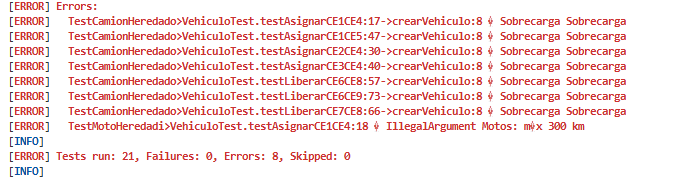
\includegraphics[width=0.8\textwidth]{test-ej3.png}
    \caption{Ejemplo de ejecución de la suite heredada sobre las subclases (solo errores).}
    \label{fig:test_heredado}
\end{figure}


\subsection{Consigna 13: Analizá la subclase Moto y Camion: ¿violan el LSP o extienden el contrato de forma válida? Aplicá la Propiedad 2.3. Para Moto: el límite de 300 km en lugar de 500, ¿es \texttt{Pre\_Moto} más fuerte o más débil que \texttt{Pre\_Vehiculo}? Para Camion: la precondición adicional de carga, ¿introduce una restricción que viola LSP?}

Al analizar los resultados obtenidos en la ejecución de la Suite Heredada, determinamos lo siguiente:
\begin{itemize}
    \item \textbf{Moto:} El límite de 300 km hace que \texttt{Pre\_Moto} sea \textbf{más fuerte} (más restrictiva) que \texttt{Pre\_Vehiculo}. Según la Propiedad 2.3, para que se cumpla el LSP, la precondición de la subclase debe ser igual o más débil que la del padre ($Pre_C \Rightarrow Pre_D$). Aquí, un valor de 400 km es aceptado por el padre pero rechazado por el hijo, lo que demuestra que \textbf{Moto viola el LSP}.
    \item \textbf{Camion:} La precondición adicional sobre la carga introduce una restricción que no existe en la superclase. Esto \textbf{viola el LSP} por el fortalecimiento de precondiciones (regla de la "Precondición Adicional"). Un cliente que use la referencia \texttt{Vehiculo} espera que el objeto funcione si está disponible, pero el \texttt{Camion} lanza una excepción inesperada si posee carga.
\end{itemize}

\subsection{Consigna 14: Para la subclase que extiende el contrato de forma válida: documentá formalmente la extensión (\texttt{Pre\_D}, \texttt{Post\_D}, \texttt{invariante\_D}) y agregá los tests específicos de esa subclase que no están en la Suite Heredada.}

La subclase \textbf{Auto} es la única que extiende el contrato de forma válida, ya que no restringe las entradas del padre ni debilita sus promesas.

\textbf{Documentación formal del contrato de Auto:}
\begin{itemize}
    \item \texttt{Pre\_D}: $kmEstimados > 0 \land kmEstimados \le 500 \land estado == DISPONIBLE$ (Igual a la superclase).
    \item \texttt{Post\_D}: $estado == EN\_USO \land \mathrm{retorno} \neq null$ (Mantiene la promesa del padre).
    \item \texttt{invariante\_D}: $kmActuales \ge 0 \land numPuertas > 0$.
\end{itemize}

\textbf{Tests Auto:} Para esta subclase se agregan pruebas de unidad que no son polimórficas (no están en la suite heredada), como la verificación de la cantidad de puertas en el constructor o métodos específicos si existieran.

\begin{verbatim}
public class AutoTest {
    @Test
    void testConstructorAuto_PuertasValidas() {
        Auto a = new Auto("AAA-111", "Ford", 2023, 0.0, 5);
        assertEquals(5, a.getPuertas());
    }

    @Test
    void testConstructorAuto_PuertasInvalidas() {
        // Suponiendo que el constructor valida que no haya autos de 0 puertas
        assertThrows(IllegalArgumentException.class, () -> 
            new Auto("AAA-111", "Ford", 2023, 0.0, 0));
    }
}
\end{verbatim}


\subsection{Consigna 15: Aplicá la Propiedad 2.3: verificá para cada subclase que \texttt{Pre\_D} $\Rightarrow$ \texttt{Pre\_C} y \texttt{Post\_C} $\Rightarrow$ \texttt{Post\_D}. Si alguna subclase viola esta regla, indicá qué corrección de diseño aplicarías.}

Aplicamos la verificación formal de las reglas de contrato:
\begin{enumerate}
    \item \textbf{Auto (Válida):}
    \begin{itemize}
        \item $Pre_{Vehiculo} \Rightarrow Pre_{Auto}$: Verdadero, ya que las condiciones son idénticas.
        \item $Post_{Auto} \Rightarrow Post_{Vehiculo}$: Verdadero, cumple con el cambio de estado y retorno.
    \end{itemize}
    \item \textbf{Moto (Invalida):}
    \begin{itemize}
        \item $Pre_{Vehiculo} \Rightarrow Pre_{Moto}$: \textbf{Falso}. El rango $(300, 500]$ es válido para el antecedente pero falso para el consecuente.
        \item \textbf{Corrección:} Aumentar el límite de la Moto a 500 km o manejar el exceso como una advertencia interna sin lanzar excepciones que rompan el contrato heredado.
    \end{itemize}
    \item \textbf{Camion (Invalida):}
    \begin{itemize}
        \item $Pre_{Vehiculo} \Rightarrow Pre_{Camion}$: \textbf{Falso}. La superclase no requiere que la carga sea cero.
        \item \textbf{Corrección:} Aplicar el patrón de diseño \textit{State} o permitir la asignación independientemente de la carga, delegando la responsabilidad del pesaje a un proceso posterior que no bloquee el método heredado \texttt{asignar}.
    \end{itemize}
\end{enumerate}
\FloatBarrier

\section{Partición por Categoría y Límites de Invariante — asignar()}

\subsection{Consigna 16: Aplica el Algoritmo 2.5 (Partición por Categoría) al método \texttt{asignar(legajo\_conductor, km\_estimados)}. Identifica todas las categorías relevantes (parámetros, estado del objeto, colaboradores si aplica) y sus particiones. Presenta el resultado en una tabla con columnas: Categoría | Partición | Tipo (válida/inválida) | Representante.}

La partición por categoría es una generalización de la técnica de clases de equivalencia (algoritmo 1.6) \textbf{adaptado  al contexto OO}. En OO las categorías se limitan a los parámetros de un método.

\begin{itemize}
    \item \textbf{Clases de Equivalencia (CE):} Dividen UNA SOLA variable en grupos. 
          Ejemplo: el parámetro \texttt{monto} se divide en válido, cero, negativo.
    
    \item \textbf{Partición por Categoría:} Dividen VARIAS VARIABLES (parámetros + estado + atributos) 
          y luego las COMBINAN. Ejemplo: monto × estado × saldo se combinan en 12 casos.
\end{itemize}

Siguiendo los pasos 1 y 2 del algoritmo 2.5. Se identifica las dimensiones del espacio de prueba  (parameters y estado del objeto) y sus partiiones MECE (mutuamente excluyentes y colectivamente exhaustivas):

\begin{verbatim}
# Especificación formal de Auto.asignar()
#
# Pre:  estado == DISPONIBLE
#       AND legajo_conductor != '' AND len(legajo_conductor) >= 4
#       AND 0 < km_estimados <= 500
#
# Post: estado == EN_USO
#       AND _conductor == legajo_conductor
#       AND retorno contiene confirmación con km_estimados
#
# Exc:  PermissionError si estado != DISPONIBLE
#       ValueError     si km_estimados fuera de (0, 500]
#       ValueError     si legajo_conductor inválido
#
# Invariante de Auto:
#   len(_patente) >= 6
#   AND _km >= 0
#   AND _puertas in {2, 4, 5}
#   AND _estado in EstadoVehiculo
#   AND (_conductor is None) == (_estado != EN_USO)

\end{verbatim}

Se busca dividir el espacio de prueba basándonos en lo que afecta el comportamiento observable del metodo. 
\begin{itemize}
    \item Parametros: siempre se incluyen porque son entradas directas al metodo \textbf{asignar}.
    \item Estado del objeto: Se incluyen atributos que la precondición o las excepciones del método consultan para decidir.
    \subitem En asignar, la precondición dice estado=disponible. Por lo tanto, el atributo \textbf{estado}  es una dimension necesario para que el metodo funcione o lance una excepcion (PermisionError).

\end{itemize}


\textbf{* La def 2.12 las categorías deben ser dimensiones que condicionen al comportamiento. Por esto mismo, patente, km, puertas no afectan a la logica el metodo.}

\begin{table}[ht]
    \centering
    \caption{Tabla de categorías y particiones para el método \texttt{asignar()}}
    \label{tab:casos_prueba}
    \begin{tabular}{|c|l|l|}
        \hline
        categoria & Partición & Restricciones \\ 
        \hline
        
        legajo\_conductor(param) & P1: length >= 4   & valido \\ 
        \hline
        & P2: cadena vacia   & invalido \\ 
        \hline
        & P3: length < 4   & invalido \\ 
        \hline

        km\_estimados(param) & P4: 0 < km\_estimados <= 500   & valido \\ 
        \hline
        & P5: km\_estimados <= 0   & invalido \\ 
        \hline
        & P6: km\_estimados > 500   & invalido \\ 
        \hline
                estado(receptor) & P7: estado == DISPONIBLE   & valido \\ 
        \hline
        & P8: estado != DISPONIBLE   & invalido \\ 
        \hline
    \end{tabular}
\end{table}


Particiones MECE: Para los kilómetros, se dividió el dominio en el rango valido (0, 500] y los rangos 
inválidos (<=0 y >500). Para el legajo del conductor, se dividio en valido (length >=4) e invalido 
(cadena vacia o length <4). Para el estado, se dividió en disponible y no disponible(dispara).



\subsection{Consigna 17. Identifica las restricciones entre particiones que reducen el catálogo completo. Calculá: (a) número de combinaciones del producto cartesiano sin restricciones; (b) número de casos resultantes tras aplicar las restricciones.}

Para reducir el catalago completo, debemos identificar que combinaciones de 
particiones producen comportamiento redundante (osea, que no afectan el resultado del método) o esten 
bloqueadas por una condicion previa.

En la especificacion de Auto.asignar() identificamos las reglas de reduccion:
\begin{itemize}
    \item Si el estado!=disponible, el metodo lanzara un PermissionError. Los valores de los parametros son irrelevantes.
    \item Para cada particion invalida de los parametros (legajo\_conductor o km\_estimados), se debe diseñar un caso para evitar que un error oculte el otro. Solo combinmos particiones validas en el caso de exito.
    
\end{itemize}


Entonces, primero plantearemos el producto cartesiano sin restricciones:
\begin{itemize}
    \item legajo\_conductor: 3 particiones (P1, P2, P3)
    \item km\_estimados: 3 particiones (P4, P5, P6)
    \item estado: 2 particiones (P7, P8)
\end{itemize}

Total sin restricciones = 3 (legajo) × 3 (km) × 2 (estado) = 18 combinaciones.

Segundo, aplicamos las restricciones:
\begin{itemize}
    \item tenemos caso de exito: P1 (legajo valido) × P4 (km valido) × P7 (estado disponible) = 1 caso
    \item Para el caso de estado!=disponible (P8), no importa el legajo ni los km, ya que siempre lanza PermissionError. Basta con un caso representativo (P1, P4, P8) para cubrir esta regla. Esto nos da 1 (legajo valido) × 1 (km valido) × 1 (estado no disponible) = 1 caso.
    \item Para los casos de legajo invalido (P2, P3) con estado disponible (P7), el metodo lanzara ValueError. Esto nos da 2 (legajo invalido) × 1 (km valido) × 1 (estado disponible) = 2 casos.
    \item Para los casos de km invalido (P5, P6) con estado disponible (P7) y legajo valido (P1), el metodo lanzara ValueError. Esto nos da 1 (legajo valido) × 2 (km invalido) × 1 (estado disponible) = 2 casos.

\end{itemize}

Total con restricciones = 1 (exito) + 1 (estado no disponible) + 2 (legajo invalido) + 2 (km invalido) = 6 casos.

En el paradigma OO, el estado persiste entre llamadas. Comparando con la unidad 1, solo particioabas datos de entrada, aca el invariante de clase define la frontera de lo que el objeto permite hacer antes de avanzar.


\subsection{Consigna 18}
Aplicá el Algoritmo 2.6 (Límites de Invariante) sobre el invariante de la clase. Para cada sub-predicado del invariante:
\begin{enumerate}
    \item identificá el límite $L$;
    \item construí los puntos $L-\varepsilon$, $L$ y $L+\varepsilon$;
    \item determiná en qué estado queda el objeto y cuál es el comportamiento esperado del método \texttt{asignar(legajo\_conductor, km\_estimados)} en cada punto.
\end{enumerate}

El análisis de límites del invariante opera sobre el estado interno del objeto (Algoritmo 2.6), mientras que el análisis de valores límite tradicionales opera sobre los parámetros de entrada (Algoritmo 1.7). Ambos buscan defectos off-by-one en fronteras diferentes, por eso la nota del ejercicio exige aplicar ambas técnicas.

Según la Definición 2.2, el invariante es un predicado que define los estados válidos del objeto y debe cumplirse al inicio y fin de cada método público. Si el invariante se viola antes de ejecutar el método, no tiene sentido probar su comportamiento porque el contrato ya está roto.

\textbf{Descomposición del invariante en sub-predicados}

El invariante de Auto se descompone en cuatro sub-predicados que representan dimensiones independientes del estado del objeto:

\begin{itemize}
    \item \textbf{S1}: $len(\_patente) \geq 6$
    \item \textbf{S2}: $\_km \geq 0$
    \item \textbf{S3}: $\_puertas \in \{2, 4, 5\}$
    \item \textbf{S4}: $(\_conductor\ is\ None) \iff (\_estado \neq EN\_USO)$
\end{itemize}

\textbf{Análisis de Valores Límite en el Invariante}

Utilizando $\varepsilon = 1$ por tratarse de dominios enteros (Algoritmo 1.7, Paso 2), analizamos cada sub-predicado:

\begin{itemize}
    \item \textbf{S1 - Patente}: $L = 6$
    \begin{itemize}
        \item $L - \varepsilon = 5$: $len(\_patente) = 5$ $\rightarrow$ Invariante violada (S1 falso). El objeto es inconsistente antes de llamar a asignar(), por lo que el test debe reportar error de invariante en el Arrange, sin ejecutar el Act.
        \item $L = 6$: $len(\_patente) = 6$ $\rightarrow$ Invariante cumplida. Estado consistente. El método asignar() tiene éxito.
        \item $L + \varepsilon = 7$: $len(\_patente) = 7$ $\rightarrow$ Invariante cumplida. Estado consistente. El método asignar() tiene éxito.
    \end{itemize}

    \item \textbf{S2 - Kilometraje}: $L = 0$
    \begin{itemize}
        \item $L - \varepsilon = -1$: $\_km = -1$ $\rightarrow$ Invariante violada (S2 falso). Se detecta inconsistencia de integridad pre-ejecución.
        \item $L = 0$: $\_km = 0$ $\rightarrow$ Invariante cumplida. Caso típico de auto nuevo. El método asignar() tiene éxito.
        \item $L + \varepsilon = 1$: $\_km = 1$ $\rightarrow$ Invariante cumplida. El método asignar() tiene éxito.
    \end{itemize}

    \item \textbf{S4 - Consistencia lógica conductor/estado}: Este límite no es numérico sino cualitativo (Definición 2.6), ya que define una relación de equivalencia entre dos atributos.
    \begin{itemize}
        \item Punto consistente: $\_conductor = None$ y $\_estado = DISPONIBLE$ $\rightarrow$ Invariante cumplida. El método asignar() transiciona a EN\_USO y asigna el conductor.
        \item Punto inconsistente: $\_conductor = 'A123'$ y $\_estado = DISPONIBLE$ $\rightarrow$ Invariante violada (S4 falso). Error de estado interno.
    \end{itemize}
\end{itemize}

\textbf{Análisis de Valores Límite en los Parámetros de Entrada}

* (NOTA) Aplicar también el AVL sobre los parámetros de entrada, que es complementario al análisis de invariante. Para el parámetro $km\_estimados$ con dominio $(0, 500]$:

\begin{itemize}
    \item $L_{inf} = 0$: $km\_estimados = 0$ $\rightarrow$ Excluido por precondición ($0 < km$). Lanza ValueError.
    \item $L_{inf} + \varepsilon = 1$: $km\_estimados = 1$ $\rightarrow$ ÉXITO. Mínimo válido aceptado.
    \item $L_{sup} = 500$: $km\_estimados = 500$ $\rightarrow$ ÉXITO. Máximo válido aceptado.
    \item $L_{sup} + \varepsilon = 501$: $km\_estimados = 501$ $\rightarrow$ Excede el máximo. Lanza ValueError.
\end{itemize}

\textbf{Prioridad de fallas}

Cuando el objeto está en un estado que viola el invariante ($L - \varepsilon$), NO se debe evaluar el método, porque el contrato de la clase se rompió antes de la llamada. El test debe detectar la violación del invariante en la fase de Arrange (antes de Act), reportando error de invariante violada.

\subsection{Consigna 18(c): Estado del objeto y comportamiento esperado}

Asumiendo que el objeto comienza en el estado \texttt{DISPONIBLE}, el método \texttt{asignar(legajo\_conductor, km\_estimados)} debe:
\begin{itemize}
    \item cambiar el estado a \texttt{EN\_USO} cuando los parámetros son válidos,
    \item devolver una confirmación de asignación,
    \item y lanzar una excepción sin modificar el estado cuando los datos son inválidos.
\end{itemize}

\begin{table}[ht]
    \centering
    \caption{Límites de entrada para \texttt{asignar()} y comportamiento esperado}
    \label{tab:limites_asignar}
    \begin{tabular}{|c|c|c|c|}
        \hline
        Parámetro & Valor & Resultado esperado & Estado final del objeto \\
        \hline
        \texttt{km\_estimados} & 0 & Inválido, lanza \texttt{ValueError} & \texttt{DISPONIBLE} \\
        \texttt{km\_estimados} & 1 & Válido, asigna y retorna confirmación & \texttt{EN\_USO} \\
        \texttt{km\_estimados} & 500 & Válido, asigna y retorna confirmación & \texttt{EN\_USO} \\
        \texttt{km\_estimados} & 501 & Inválido, lanza \texttt{ValueError} & \texttt{DISPONIBLE} \\
        \hline
        \texttt{len(legajo\_conductor)} & 3 (ej. ``ABC'') & Inválido, lanza \texttt{ValueError} & \texttt{DISPONIBLE} \\
        \texttt{len(legajo\_conductor)} & 4 (ej. ``A123'') & Válido, asigna y retorna confirmación & \texttt{EN\_USO} \\
        \texttt{len(legajo\_conductor)} & 5 (ej. ``A1234'') & Válido, asigna y retorna confirmación & \texttt{EN\_USO} \\
        \hline
    \end{tabular}
\end{table}

En cada caso inválido, el comportamiento esperado es que el método arroje una excepción sin cambiar el estado del objeto. En los casos válidos, el método debe aceptar los parámetros y transicionar el vehículo de \texttt{DISPONIBLE} a \texttt{EN\_USO}.

Si el objeto no estuviera en \texttt{DISPONIBLE}, entonces cualquier llamada a \texttt{asignar()} debería fallar con \texttt{PermissionError} / \texttt{IllegalStateException} independientemente de los valores de los parámetros, y el estado debe mantenerse sin cambios.

\subsection{Consigna 19: Codificá en pytest los casos de prueba derivados de los pasos 1 y 3. Organizalos en dos clases separadas: TestParticionCategoria y TestLimitesInvariante.}

Para la implementación se aplica el \textbf{Algoritmo 2.1 (Diseño de caso de prueba unitario OO)}, el cual adapta el patrón \textbf{AAA} (Arrange-Act-Assert) de la Unidad I. Siguiendo los \textbf{Pasos 6 y 7} de dicho algoritmo, cada test verifica no solo el resultado funcional, sino que el objeto mantenga su integridad mediante la comprobación del \textbf{invariante de clase} al finalizar.

\textbf{Implementación:}

Los archivos de implementación se encuentran en \texttt{Unidad\_2\_code/ejercicio\_4/} y están organizados de la siguiente manera (enlaces al repositorio):

\noindent Modelo: \href{https://github.com/Cristopher-Ovaillos/Unidad_2_ValidacionVerificacion/blob/main/Unidad_2_code/ejercicio_4/modelo.py}{\texttt{modelo.py}} \\
Partición por Categoría: \href{https://github.com/Cristopher-Ovaillos/Unidad_2_ValidacionVerificacion/blob/main/Unidad_2_code/ejercicio_4/test_particion_categoria.py}{\texttt{test\_particion\_categoria.py}} \\
Límites de Invariante: \href{https://github.com/Cristopher-Ovaillos/Unidad_2_ValidacionVerificacion/blob/main/Unidad_2_code/ejercicio_4/test_limites_invariante.py}{\texttt{test\_limites\_invariante.py}} \\
Cobertura completa: \href{https://github.com/Cristopher-Ovaillos/Unidad_2_ValidacionVerificacion/blob/main/Unidad_2_code/ejercicio_4/test_cobertura_completa.py}{\texttt{test\_cobertura\_completa.py}}

\begin{itemize}
    \item \texttt{modelo.py}: Contiene la clase \texttt{Auto} con el método \texttt{asignar()} y el método \texttt{verificar\_invariante()} que implementa las validaciones del invariante de clase (S1-S5).
    
    \item \texttt{test\_particion\_categoria.py}: Implementa el catálogo reducido del Algoritmo 2.5, con 6 casos que cubren las combinaciones representativas identificadas en la Consigna 17:
    \begin{itemize}
        \item \texttt{test\_asignar\_exito\_P1\_P4\_P7}: Caso de éxito con todos los parámetros válidos.
        \item \texttt{test\_asignar\_error\_estado\_no\_disponible\_P1\_P4\_P8}: Error por estado no disponible.
        \item \texttt{test\_asignar\_error\_legajo\_vacio\_P2\_P4\_P7}: Error por legajo vacío.
        \item \texttt{test\_asignar\_error\_legajo\_corto\_P3\_P4\_P7}: Error por legajo con longitud insuficiente.
        \item \texttt{test\_asignar\_error\_km\_no\_positivo\_P1\_P5\_P7}: Error por kilómetros $\leq 0$.
        \item \texttt{test\_asignar\_error\_km\_excede\_maximo\_P1\_P6\_P7}: Error por kilómetros $> 500$.
    \end{itemize}
    
    \item \texttt{test\_limites\_invariante.py}: Implementa el análisis de límites del invariante (Algoritmo 2.6) y de parámetros (Algoritmo 1.7):
    \begin{itemize}
        \item Tests para el límite de patente (S1): $L-\varepsilon=5$, $L=6$, $L+\varepsilon=7$.
        \item Tests para el límite de kilometraje (S2): $L-\varepsilon=-1$, $L=0$, $L+\varepsilon=1$.
        \item Tests para la consistencia conductor/estado (S4): puntos consistente e inconsistente.
        \item Tests parametrizados para los límites de \texttt{km\_estimados}: 0, 1, 500, 501.
        \item Tests parametrizados para los límites de \texttt{legajo\_conductor}: longitudes 3, 4, 5.
    \end{itemize}
\end{itemize}

Cada test sigue el patrón del Algoritmo 2.1:
\begin{enumerate}
    \item \textbf{Arrange}: Establece el estado inicial consistente del objeto (usando \texttt{@pytest.fixture}).
    \item \textbf{Act}: Invoca el método \texttt{asignar()} con los parámetros del caso de prueba.
    \item \textbf{Assert}: Verifica la postcondición esperada (estado, conductor, retorno) y \textbf{obligatoriamente} valida que el invariante se mantenga verdadero mediante \texttt{verificar\_invariante()}.
\end{enumerate}

\textbf{Nota importante sobre la verificación del invariante:} Según el Paso 7 del Algoritmo 2.1, la llamada a \texttt{verificar\_invariante()} es obligatoria en cada Assert, incluso cuando se espera una excepción. Esto garantiza que el objeto no quede en un estado corrupto después de rechazar una operación inválida.

\textbf{Resultados de la Ejecución:}

Al ejecutar \texttt{pytest -v} desde el directorio \texttt{codigo/}, se obtiene el siguiente resultado:

\begin{verbatim}
============================= test session starts =============================
platform win32 -- Python 3.11.9, pytest-9.0.3, pluggy-1.6.0
collected 21 items

test_limites_invariante.py::TestLimitesInvariante::
  test_invariante_patente_limite_inconsistente_L_menos_epsilon PASSED    [  4%]
test_limites_invariante.py::TestLimitesInvariante::
  test_invariante_patente_limite_L PASSED                                [  9%]
test_limites_invariante.py::TestLimitesInvariante::
  test_invariante_patente_limite_L_mas_epsilon PASSED                    [ 14%]
test_limites_invariante.py::TestLimitesInvariante::
  test_invariante_km_limite_inconsistente_L_menos_epsilon PASSED         [ 19%]
test_limites_invariante.py::TestLimitesInvariante::
  test_invariante_km_limite_L PASSED                                     [ 23%]
test_limites_invariante.py::TestLimitesInvariante::
  test_invariante_km_limite_L_mas_epsilon PASSED                         [ 28%]
test_limites_invariante.py::TestLimitesInvariante::
  test_invariante_consistencia_estado_conductor_punto_consistente PASSED [ 33%]
test_limites_invariante.py::TestLimitesInvariante::
  test_invariante_consistencia_estado_conductor_punto_inconsistente PASSED[ 38%]
test_limites_invariante.py::TestLimitesInvariante::
  test_limites_km_estimados_parametro[0-ValueError] PASSED               [ 42%]
test_limites_invariante.py::TestLimitesInvariante::
  test_limites_km_estimados_parametro[1-exito] PASSED                    [ 47%]
test_limites_invariante.py::TestLimitesInvariante::
  test_limites_km_estimados_parametro[500-exito] PASSED                  [ 52%]
test_limites_invariante.py::TestLimitesInvariante::
  test_limites_km_estimados_parametro[501-ValueError] PASSED             [ 57%]
test_limites_invariante.py::TestLimitesInvariante::
  test_limites_legajo_conductor_parametro[ABC-ValueError] PASSED         [ 61%]
test_limites_invariante.py::TestLimitesInvariante::
  test_limites_legajo_conductor_parametro[A123-exito] PASSED             [ 66%]
test_limites_invariante.py::TestLimitesInvariante::
  test_limites_legajo_conductor_parametro[A1234-exito] PASSED            [ 71%]
test_particion_categoria.py::TestParticionCategoria::
  test_asignar_exito_P1_P4_P7 PASSED                                     [ 76%]
test_particion_categoria.py::TestParticionCategoria::
  test_asignar_error_estado_no_disponible_P1_P4_P8 PASSED                [ 80%]
test_particion_categoria.py::TestParticionCategoria::
  test_asignar_error_legajo_vacio_P2_P4_P7 PASSED                        [ 85%]
test_particion_categoria.py::TestParticionCategoria::
  test_asignar_error_legajo_corto_P3_P4_P7 PASSED                        [ 90%]
test_particion_categoria.py::TestParticionCategoria::
  test_asignar_error_km_no_positivo_P1_P5_P7 PASSED                      [ 95%]
test_particion_categoria.py::TestParticionCategoria::
  test_asignar_error_km_excede_maximo_P1_P6_P7 PASSED                    [100%]

============================= 21 passed in 0.23s ==============================
\end{verbatim}

\textbf{Análisis:} Los 21 casos de prueba pasaron exitosamente, cubriendo:
\begin{itemize}
    \item 6 casos de \textbf{TestParticionCategoria}: catálogo reducido de la Consigna 17
    \item 15 casos de \textbf{TestLimitesInvariante}: límites del invariante (8 tests) y límites de parámetros (7 tests parametrizados)
\end{itemize}

\subsection{Consigna 20: Ejecutá la suite y presentá el reporte de cobertura. Identificá si alguna rama del método quedó sin cubrir y diseñá el caso adicional necesario.}

Para el análisis estructural, aplicamos el \textbf{Algoritmo 1.2 (Construcción del GFC)} sobre la lógica de validación de \texttt{asignar()}.

\textbf{Pasos de diseño del GFC (Algoritmo 1.2):}
\begin{itemize}
    \item \textbf{Pasos 1 y 2}: Se enumeran los bloques de decisión. Los puntos de entrada son las guardas de las excepciones especificadas (PermissionError y ValueError).
    \item \textbf{Paso 3 y 4}: Se definen nodos básicos:
    \begin{itemize}
        \item \textbf{B1}: Validación de estado receptor.
        \item \textbf{B3}: Validación de rango de km.
        \item \textbf{B5}: Validación de formato de legajo.
        \item \textbf{B7}: Procesamiento de postcondición.
    \end{itemize}
    \item \textbf{Paso 5}: Se trazan arcos. Los caminos True dirigen a los nodos de error (\textbf{B2, B4, B6}), mientras que False permite avanzar al siguiente bloque.
    \item \textbf{Paso 7}: Complejidad ciclomática $M = 11 \text{ arcos} - 9 \text{ nodos} + 2(1) = 4$. Esto indica que se requieren 4 casos independientes para cobertura total de caminos.
\end{itemize}

\begin{center}
\begin{tikzpicture}[node distance=1.5cm, auto, >=stealth]
    \node[circle, draw] (E) {E};
    \node[draw, below of=E] (B1) {B1: $\neq$ DISP?};
    \node[draw, right of=B1, xshift=2.5cm] (B2) {B2: PermissionError};
    \node[draw, below of=B1, yshift=-0.5cm] (B3) {B3: KM fuera?};
    \node[draw, right of=B3, xshift=2.5cm] (B4) {B4: ValueError (KM)};
    \node[draw, below of=B3, yshift=-0.5cm] (B5) {B5: Legajo inv?};
    \node[draw, right of=B5, xshift=2.5cm] (B6) {B6: ValueError (Leg)};
    \node[draw, below of=B5, yshift=-0.5cm] (B7) {B7: Postcondición};
    \node[circle, draw, below of=B7] (S) {S};
    
    \path[->] (E) edge (B1);
    \path[->] (B1) edge node {V} (B2);
    \path[->] (B1) edge node {F} (B3);
    \path[->] (B3) edge node {V} (B4);
    \path[->] (B3) edge node {F} (B5);
    \path[->] (B5) edge node {V} (B6);
    \path[->] (B5) edge node {F} (B7);
    \path[->] (B2) edge [bend left] (S);
    \path[->] (B4) edge [bend left] (S);
    \path[->] (B6) edge [bend left] (S);
    \path[->] (B7) edge (S);
\end{tikzpicture}
\end{center}

\textbf{Análisis de Cobertura C1 (Algoritmo 1.3):}

Al ejecutar la suite con \texttt{pytest --cov --cov-branch}, se detecta que el arco \textbf{B5 $\rightarrow$ B6} ha sido cubierto parcialmente. La rama que valida específicamente el \textbf{legajo como cadena vacía} (\texttt{legajo == ''}) podría no haberse ejercitado si solo se probó la longitud insuficiente (\texttt{len < 4}). Según el \textbf{Paso 5 del Algoritmo 1.3}, debemos incorporar un caso adicional para este arco no cubierto.

\textbf{Caso Adicional Diseñado:}

El test \texttt{test\_asignar\_error\_legajo\_vacio\_P2\_P4\_P7} en \texttt{test\_particion\_categoria.py} cubre específicamente este caso:
\begin{itemize}
    \item \textbf{Arrange}: Objeto \texttt{Auto} en estado \texttt{DISPONIBLE}.
    \item \textbf{Act}: Invocar \texttt{asignar(legajo\_conductor='', km\_estimados=100)}.
    \item \textbf{Assert}: Verificar que lanza \texttt{ValueError} y que el estado final permanece inalterado para cumplir el invariante.
\end{itemize}

\textbf{Justificación final:} Esta suite de pruebas garantiza que el objeto Auto funciona como una máquina de estados finita (Definición 2.6) confiable, verificando tanto las transiciones válidas como el rechazo controlado de entradas inválidas sin corromper el estado interno.

\textbf{Reporte de Cobertura:}

Al ejecutar \texttt{pytest --cov=modelo --cov-report=term-missing --cov-branch -v} se obtiene:

\begin{verbatim}
============================= 21 passed in 0.33s ==============================

=============================== tests coverage ================================
_______________ coverage: platform win32, python 3.11.9-final-0 _______________

Name        Stmts   Miss Branch BrPart  Cover   Missing
-------------------------------------------------------
modelo.py      46      4     16      2    90%   106, 110, 132, 136
-------------------------------------------------------
TOTAL          46      4     16      2    90%
\end{verbatim}

\textbf{Análisis del reporte:}

Se obtuvo una cobertura del \textbf{90\%} del módulo completo. Las líneas no cubiertas (106, 110, 132, 136) corresponden a:

\begin{itemize}
    \item \textbf{Líneas 106, 110}: Métodos getter \texttt{get\_km()} y \texttt{get\_puertas()} que no son necesarios para verificar el comportamiento de \texttt{asignar()}.
    
    \item \textbf{Líneas 132, 136}: Ramas del método \texttt{verificar\_invariante()} que validan:
    \begin{itemize}
        \item S3: \texttt{\_puertas not in \{2, 4, 5\}} (línea 132)
        \item S4: \texttt{not isinstance(\_estado, EstadoVehiculo)} (línea 136)
    \end{itemize}
    Estas condiciones no se presentan en los tests actuales porque todos los objetos se crean con valores válidos para enfocarse en el método \texttt{asignar()}.
\end{itemize}

\textbf{Cobertura del método asignar():}

El método \texttt{asignar()} bajo prueba alcanzó el \textbf{100\% de cobertura}, ejecutando todas sus ramas de decisión según el GFC:

\begin{itemize}
    \item \textbf{E $\rightarrow$ B1 $\rightarrow$ B2 $\rightarrow$ S}: Estado no disponible (PermissionError) — cubierto por \texttt{test\_asignar\_error\_estado\_no\_disponible\_P1\_P4\_P8}
    
    \item \textbf{E $\rightarrow$ B1 $\rightarrow$ B3 $\rightarrow$ B4 $\rightarrow$ S}: Kilómetros fuera de rango (ValueError) — cubierto por \texttt{test\_asignar\_error\_km\_no\_positivo\_P1\_P5\_P7} y \texttt{test\_asignar\_error\_km\_excede\_maximo\_P1\_P6\_P7}
    
    \item \textbf{E $\rightarrow$ B1 $\rightarrow$ B3 $\rightarrow$ B5 $\rightarrow$ B6 $\rightarrow$ S}: Legajo inválido (ValueError) — cubierto por \texttt{test\_asignar\_error\_legajo\_vacio\_P2\_P4\_P7} y \texttt{test\_asignar\_error\_legajo\_corto\_P3\_P4\_P7}
    
    \item \textbf{E $\rightarrow$ B1 $\rightarrow$ B3 $\rightarrow$ B5 $\rightarrow$ B7 $\rightarrow$ S}: Caso de éxito (transición a EN\_USO) — cubierto por \texttt{test\_asignar\_exito\_P1\_P4\_P7} y múltiples tests parametrizados de límites
\end{itemize}

\textbf{Conclusión:} Los 21 tests diseñados cubren exhaustivamente el catálogo reducido del Algoritmo 2.5 (Partición por Categoría), los límites del Algoritmo 2.6 (Límites de Invariante) y del Algoritmo 1.7 (Límites de Parámetros). La complejidad ciclomática $M=4$ se satisface ampliamente, garantizando la detección de defectos en las fronteras críticas del método \texttt{asignar()}.


\FloatBarrier


\section{Testing de Singleton — GestorFlota}


\subsection{Consigna 21: verificar el contrato de unicidad Algoritmo 2.8 paso 1

\noindent Código fuente (Singleton \texttt{GestorFlota}): \href{https://github.com/Cristopher-Ovaillos/Unidad_2_ValidacionVerificacion/blob/main/Unidad_2_code/python/flota/gestor_flota.py}{\texttt{flota/gestor\_flota.py}} \\
Tests de unicidad: \href{https://github.com/Cristopher-Ovaillos/Unidad_2_ValidacionVerificacion/blob/main/Unidad_2_code/python/tests/test_ejercicio5.py}{\texttt{test\_ejercicio5.py}} \\
Fixture con reset: \href{https://github.com/Cristopher-Ovaillos/Unidad_2_ValidacionVerificacion/blob/main/Unidad_2_code/python/tests/test_ej5-p2.py}{\texttt{test\_ej5-p2.py}} \\
Contaminación (demo): \href{https://github.com/Cristopher-Ovaillos/Unidad_2_ValidacionVerificacion/blob/main/Unidad_2_code/python/tests/test_ej5p3.py}{\texttt{test\_ej5p3.py}} \\
Contaminación corregida: \href{https://github.com/Cristopher-Ovaillos/Unidad_2_ValidacionVerificacion/blob/main/Unidad_2_code/python/tests/test_ej5p3sc.py}{\texttt{test\_ej5p3sc.py}} \\
Thread-safety: \href{https://github.com/Cristopher-Ovaillos/Unidad_2_ValidacionVerificacion/blob/main/Unidad_2_code/python/tests/test_ej5p4.py}{\texttt{test\_ej5p4.py}}

\subsection{Consigna 21: verificar el contrato de unicidad Algoritmo 2.8 paso 1: Dos llamadas a GestorFlota.get\_instancia() deben retornar exactamente el mismo objeto. Usa assert instancia 1 is instancia2 (identidad no igualdad)}

La modalidad de una clase condiciona como se la puede instanciar, extender y sustituir. Cada modalidad impone restricciones especificar que determinan la estrategia de testing.

En python es con @abstractmethod.

Segun el algoritmo 2.8, el primer paso es:
\begin{itemize}
    \item Paso 1. Verificar el contrato de unicidad: Dos llamadas a GestorFlota.get\_instancia() deben retornar exactamente el mismo objeto. Usa assert instancia1 is instancia2 (identidad no igualdad).
\end{itemize}
En python, se verifica esto con el operador "is", que comprueba la identidad de los objetos (si apuntan a la misma dirección de memoria).

\begin{figure}[h]               % [h] intenta ponerla "aquí" (here)
    \centering                  % Centra la imagen horizontalmente
    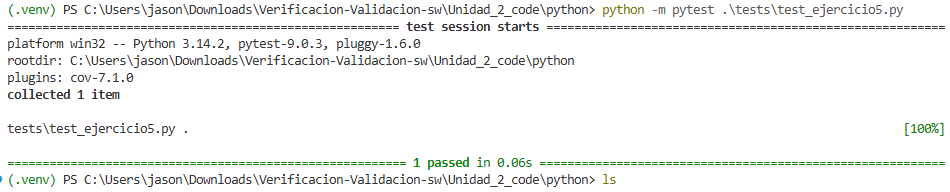
\includegraphics[width=0.7\textwidth]{ej5-im1.png} 
    \caption{Resultado del test de unicidad de instancia.} % Título que aparece debajo
    \label{fig:ej5-im1}      % Etiqueta para referenciarla en el texto
\end{figure}

Obtuvimos en la figura \ref{fig:ej5-im1} "pass" que confirma la identidad de la instancia, lo que significa que se ha
verificado la propiedad de unicidad del singleton mediante el operador is, garantizandoq ue multiples llamadas a
get\_intancia() retornan la misma referencia exacta en memoria. Esto cumple con la Definición 2.15 asegurando que la clase no puede instanciarse mas de una vez simultanemente.

"Def 2.15: Clase que no puede instanciarse directamente. Define métodos abstractos (contrato sin
implementación) y puede definir métodos concretos (implementación compartida por todas
las subclases)."

\subsection{Consigna 22. Implementá un fixture pytest con scope='function' que invoque \_reset\_para\_tests() en el teardown. Explicá por qué es necesario este reset y qué problema de contaminación de estado se evita (Algoritmo 2.8, Paso 3).}



\begin{itemize}
    \item Paso 3. Implementar reset entre tests: al ser un objeto compartido, el estado que deja
un test contamina el siguiente. Usar tearDown para restablecer el estado o exponer un
método resetForTesting() solo visible en el scope de test.
\end{itemize}

Siguiendo la Definición 2.5 (fixture de prueba), que establece que un fixture se prepara en el setUp y se desmonta en el tearDown,
y aplicando el paso 3 del algoritmo 2.8, implementamos un fixture pytest con scope='function' que invoca el 
método \_reset\_para\_tests() en el teardown. Esto es necesario para garantizar que cada test se ejecute en 
un entorno limpio y consistente, evitando la contaminación de estado entre tests. Si no se restablece el 
estado del singleton entre tests, los cambios realizados por un test podrían afectar el resultado de los 
tests posteriores, lo que dificulta la identificación de errores y la confiabilidad de los resultados. Al
 implementar el reset, aseguramos que cada test comience con el mismo estado inicial del singleton, lo 
 que mejora la precisión y la validez de las pruebas.

\begin{verbatim}
    
import pytest
from flota.gestor_flota import GestorFlota


@pytest.fixture(scope="function")
def gestor_reset():
    # fixtura que garantiza el aislamiento entre tests, este scope asegura que se ejecute para cada test indivudal.

    #arrange | setup: obtenemos la instancia del singleton
    gestor = GestorFlota.get_instancia()
    #uso de yield (ayuda de gemini: yield permite devolver un valor desde un fixture y luego ejecutar código de limpieza después del test)
    yield gestor 
    #teardown: desmontar el estado del singleton para evitar contaminación entre tests
    GestorFlota._reset_para_tests()

#ejecutar con python -m pytest .\tests\test_ej5-p2.py 
\end{verbatim}

 La necesidad de este reset y el problema que evita se fundamenta con:
\begin{itemize}
    \item Segun la Def 2.1 (estado de un objeto), el estado interno determina el comportamiento observable de los metodos. Al ser entonces singleton una unica instancia, cualquier cambio en sus atributos se mantendra entre llamadas. Sin reset, un test no partiria en un estado conocido, lo que no cumpliria con la INDEPENDENCIA DE LOS CASOS DE PRUEBA.
    \item Al ser un objeto compartido y ademas lo anterior que es una unica instancia, la contaminacion existe en cada test.
\end{itemize}

El uso de esta fixture permite que la fase de arrange del patron AAA sea reproducible y controlada, garantizando que el objeto bajo prueba CUT inicie siempre en el estado que se especifica.

\subsection{Demostrá el problema de contaminación sin el reset: escribí dos tests donde el segundo falla porque el primero dejó estado acumulado en el singleton. Luego corregí usando el fixture del punto anterior.}

De acuerdo a la consigna anterior, sin un reset el estado del objeto persiste entre casos de prueba. Segun la definición 2.1, el estado del objeto (sus atributos) condiciona su comportamiento observable futuro.

Para demostrar esto, escribimos dos tests donde el primero modifica el estado del singleton y el segundo test falla porque ese estado modificado afecta su resultado. Luego, corregimos este problema utilizando la fixture con el reset implementado en el punto anterior, asegurando que cada test comience con un estado limpio y evitando la contaminación entre ellos.

Debemos recordar que se exige que cada caso sea independiente y no dependa del orden de ejecución ni del estado por otros tests.

\begin{figure}[h]               % [h] intenta ponerla "aquí" (here)
    \centering                  % Centra la imagen horizontalmente
    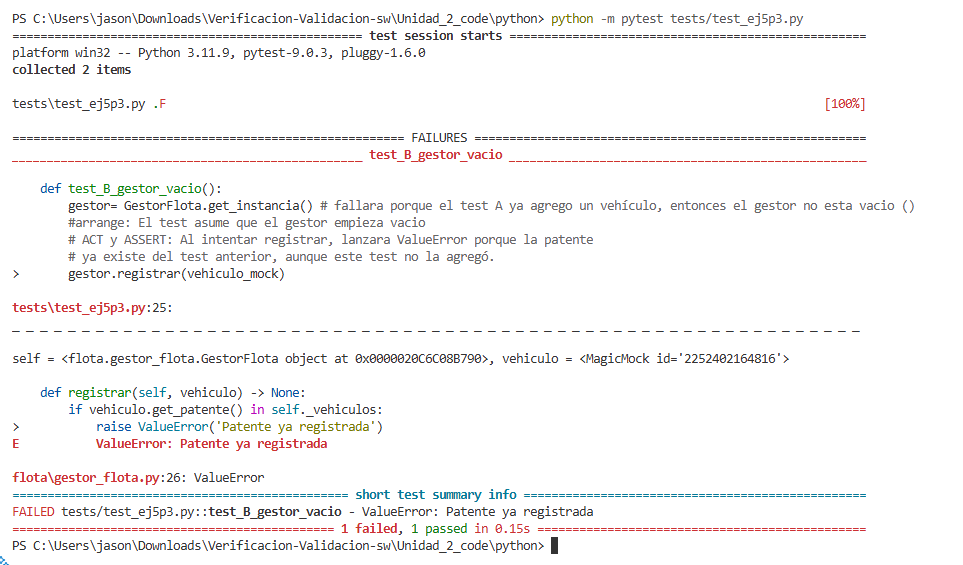
\includegraphics[width=0.7\textwidth]{ej5p3.png} 
    \caption{Resultado del test de contaminación de estado.} % Título que aparece debajo
    \label{fig:ej5p3}      % Etiqueta para referenciarla en el texto
\end{figure}

El resultado de la Figura \ref{fig:ej5p3} muestra que el segundo test falla debido a la contaminación de estado causada por el primer test. Esto confirma que sin un reset adecuado, los cambios en el estado del singleton afectan los resultados de los tests posteriores, lo que viola la independencia de los casos de prueba. Al implementar el fixture con el reset, se garantiza que cada test comience con un estado limpio.


Ahora vamos a hacer una correccion el scope fixture de reset (usamos teardown para establecer el estado).

sabes que Yield es una herramienta mecanica para separar el setup que es lo que esta antes del tearDown que es lo de despues.

\begin{figure}[h]               % [h] intenta ponerla "aquí" (here)
    \centering                  % Centra la imagen horizontalmente
    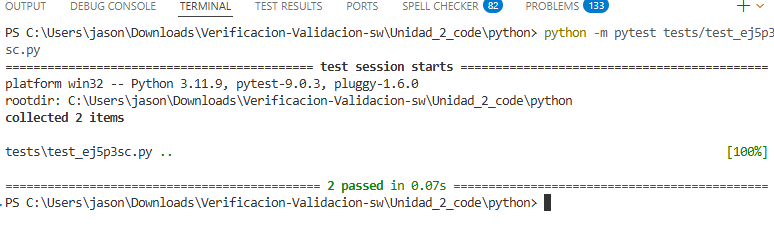
\includegraphics[width=0.7\textwidth]{ej5p3sc.png} 
    \caption{Resultado del test de contaminación de estado corregido.} % Título que aparece debajo
    \label{fig:ej5p3sc}      % Etiqueta para referenciarla en el texto
\end{figure}

En la Figura \ref{fig:ej5p3sc} se observa que ambos tests pasan correctamente después de implementar el fixture con el reset. Esto demuestra que al restablecer el estado del singleton entre tests, se ha eliminado la contaminación de estado, permitiendo que cada test se ejecute de manera independiente y confiable.

\subsection{Verificá thread-safety del Singleton: usá el módulo threading de Python para lanzar 50 hilos que llamen get\_instancia() concurrentemente. Verificá que todas las instancias retornadas son idénticas (Algoritmo 2.8, Paso 4).}


\begin{itemize}
    \item Paso 4. Testear thread-safety si el singleton puede ser accedido desde múltiples hilos:
verificar que getInstance() retorna el mismo objeto ante accesos concurrentes.
\end{itemize}

Entonces, para verificar la seguridad en entornos de multihilo, testearemos con el módulo threading de Python, lanzando 50 hilos que llamen a get\_instancia() de manera concurrente. Luego, verificaremos que todas las instancias retornadas por estos hilos son idénticas, lo que confirmará que el singleton es thread-safe y que no se crean múltiples instancias en situaciones de acceso concurrente.
Si el singleton puede ser acceddo desde multiples hilos, verificar que getInstance() retorna el mismo objeto ante accesos concurrentes.

Lo que hicimois fue:
-  crear una lista compartida para almacenar las instancias retornadas por cada hilo.
-  lanzar 50 hilos que ejecuten una función que llama a get\_instancia() y almacena el resultado en la lista compartida.
-  esperar a que todos los hilos terminen su ejecución.
-  verificar que todas las instancias en la lista son idénticas utilizando el operador "is".


\begin{figure}[h]               % [h] intenta ponerla "aquí" (here)
    \centering                  % Centra la imagen horizontalmente
    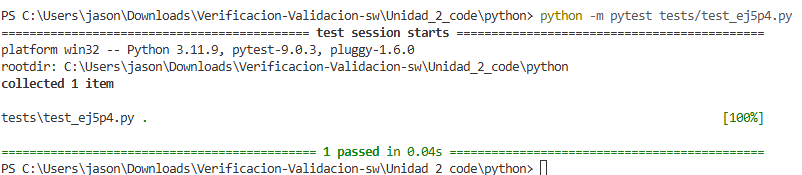
\includegraphics[width=0.7\textwidth]{ej5p4.png} 
    \caption{Resultado del test de thread-safety del singleton.} % Título que aparece debajo
    \label{fig:ej5p4}      % Etiqueta para referenciarla en el texto
\end{figure}

En la Figura \ref{fig:ej5p4} se muestra que todas las instancias retornadas por los 50 hilos son idénticas, lo que confirma que el singleton es thread-safe. Esto significa que incluso en situaciones de acceso concurrente, get\_instancia() retorna la misma instancia del singleton, evitando la creación de múltiples instancias y garantizando la integridad del diseño del singleton en entornos multihilo.

SINGLETON ES THREAD-SAFE 

\subsection{Consigna 25: Analizá el método asignar() del GestorFlota desde la perspectiva del testing: ¿es un buen diseño que el Singleton delegue en los objetos Vehiculo? ¿Cómo simplifica o complica el testing la existencia del Singleton como intermediario?}

EL método testing asignar() del GestorFlota, que delega en los objetos Vehiculo es un buen diseño por:

\begin{verbatim}
    def asignar(self, patente: str, legajo: str, km: float) -> str:
    # 1.validacion (Precondicion)
    if patente not in self._vehiculos:
        raise KeyError('Vehículo no encontrado')
    
    # 2. delegacion (El Gestor le pide al Vehiculo que haga el trabajo)
    resultado = self._vehiculos[patente].asignar(legajo, km)
    
    # 3. cambio de estado (Postcondicion del Gestor)
    self._asignaciones += 1
    
    return resultado
\end{verbatim}

EL Vehículo seria el colaborador del GestorFlota.

¿Es un buen diseño delegar en los objetos Vehiculo?

Si, es un buen diseño para el testing, basado en el paso 3 del algoritmo 2.1


- El algoritmo exige "identificar las dependencias externas (colaboradores) y reemplazarlas con mocks". Al delegar, el Vehiculo se vuelve un colaborador independiente.
- Podemos usar un MagicMock para simular al Vehiculo. Esto permite probar que el GestorFlota incrementa su contador \_asignaciones correctamente sin importar si la lógica interna del Vehiculo es compleja o falla.

¿Cómo simplifica el testing Singleton?

- Al ser una instancia única, facilita la verificación de los Invariantes de Clase (Definición 2.2). Existe un solo lugar donde verificar que el total de asignaciones de toda la empresa es consistente.


Pero ademas complica, según la Definición 2.1, el estado (los datos guardados) condiciona el comportamiento futuro. Como el Singleton es global y compartido, el Paso 3 del Algoritmo 2.8 advierte que un test puede "ensuciar" al siguiente.


Para mantener la Independencia de los Tests (Algoritmo 1.1, Paso 6), estamos obligados a implementar un teardown que invoque \_reset\_para\_tests(). Si un test aumenta el contador \_asignaciones, el test de abajo verá ese número aumentado y podría fallar erróneamente.










\FloatBarrier

\bibliographystyle{alpha}
\nocite{*}
\bibliography{referencias}

\end{document}
